\chapter{Helixantenne}
Die zweite aufgebaute Antenne ist eine monofilare Helixantenne. Dieser Antennentyp ist gerichtet, was bedeutet, dass sie in eine bestimmte Richtung einen höheren Antennengewinn als in andere Richtungen hat. Sie ist eine der einfachsten Antennenarten um eine zirkulare Polarisation zu erzielen. Kombiniert mit ihrer hohen Bandbreite macht sie das zu einer attraktiven Option zum Nachbau und zur Verwendung in der Satellitenkommunikation. \cite{helixWebsite}

Für die in dieser Diplomarbeit konstruierte Helixantenne wurden die folgenden Vorgaben gewählt.

\begin{center}
	\begin{tabular}{|c|c|}
	\textbf{Parameter} & \textbf{Wert}\\
	Resonanzfrequenz & 433MHz\\
	Windungen & 6\\
	Abstand zwischen Windungen & $0,25\lambda$\\
	Polarisationsart & RHCP\\
	Betriebsmodus & Axial-Modus
\end{tabular}
\end{center}

Wobei $"$RHCP$"$ $"$Right Hand Circularily Polarized$"$ bedeutet. Für mehr Informationen zur zirkularen Polarisation wird auf den Abschnitt $"$\ref{subsec:pol} Polarisation$"$ verwiesen.

\section{Design}
Durch den Einsatz im Freien muss die Helixantenne einige Anforderungen erfüllen. Beispielsweise dürfen wichtige Strukturelemente unter UV-Einwirkung nicht brüchig werden, es darf sich durch Regen kein Wasser stauen und sie muss starkem Wind standhalten. 

Um die Helixantenne zu designen wurden Online-Rechner verwendet \cite{calculator_daycounter, calculator_jcoppens}.

\begin{center}
	\begin{tabular}{|c|c|}
	\textbf{Parameter} & \textbf{Wert} \\
	Wellenlänge &  692.8mm\\
	Durchmesser (intern) & 235.7mm\\
	Abstand zwischen den Windungen & 173.2mm\\
	Gesamthöhe & 1039.2mm\\
	minimaler Reflektor-Durchmesser & 429.5mm
\end{tabular}
\end{center}

Mithilfe dieser Werte wurde die erste Wendelantenne in Fusion 360 konstruiert. 

\begin{figure}[h!]
	\centering
	\includegraphics[width=5cm]{../ref/Erste Helixnäherung v0.png}
	\label{fig:ersteHelixnäherung}
	\caption{Das CAD-Modell für die Helixantenne mit den berechneten Werten}
\end{figure}

Diese wurde mithilfe von CENOS-Simulation-Suite für einen Frequenzbereich von [FREQUENZBEREICH] simuliert. Die Ergebnisse gaben Aufschluss über die Performance der Antenne in einer idealen Umgebung.

S11-Parameter
SWR
Abstrahlverhalten 2D
Abstrahlverhalten 3D

Es wurde der Schluss gezogen, dass die Resonanzfrequenz zu weit über dem gewünschten Wert von 433MHz liegt. Diese lässt sich durch Veränderung des Durchmessers der Spirale oder des Abstandes zwischen den Windungen verändern.

Durch das Abändern des Durchmessers konnte die gewünschte Resonanzfrequenz von 433MHz mit einem Helix-Durchmesser von 270mm erreicht werden. Der Reflektor wurde aus der Theorie mit ca. $\frac{3\lambda}{4}$ festgelegt \cite{Kraus-2002-AntennasB}, was einem Durchmesser von ungefähr 520mm entspricht.

Es ist wichtig anzumerken, dass der Steigungswinkel der Spirale hierbei ca. 11,5° beträgt. Dies bedeutet, dass die Steigung von dem relativ engen Idealbereich zwischen 12° und 14° abweicht.

\section{Realisierung}
Die Helixantenne benötigt zur Funktion nur zwei Bauteile: die Spirale und der Reflektor. Für die Simulation genügt dieses Modell, allerdings werden in der Realität Strukturelemente benötigt um diese zu befestigen.

\begin{figure}[H]
	\centering
	\includegraphics[width=10cm,angle=270]{../ref/Helixantenne-real.jpg}
	\caption{Reale Helixantenne}
	\label{fig:helix-real}
\end{figure}

MATERIALLISTE

\begin{itemize}
	\item PVC-Rohr
	\item Abstandhalter (Teflon bzw. PAS60)
	\item Rohrflansch
	\item Aluminiumrohr
	\item Aluminiumplatte
\end{itemize}

Das schwarze PVC-Stützrohr ist UV-stabilisiert. Wäre der Kunststoff nicht gegen UV-Strahlung geschützt, so würde dieser nach einer Zeit spröde und strukturell unzuverlässig.

\begin{figure}[H]
	\centering
	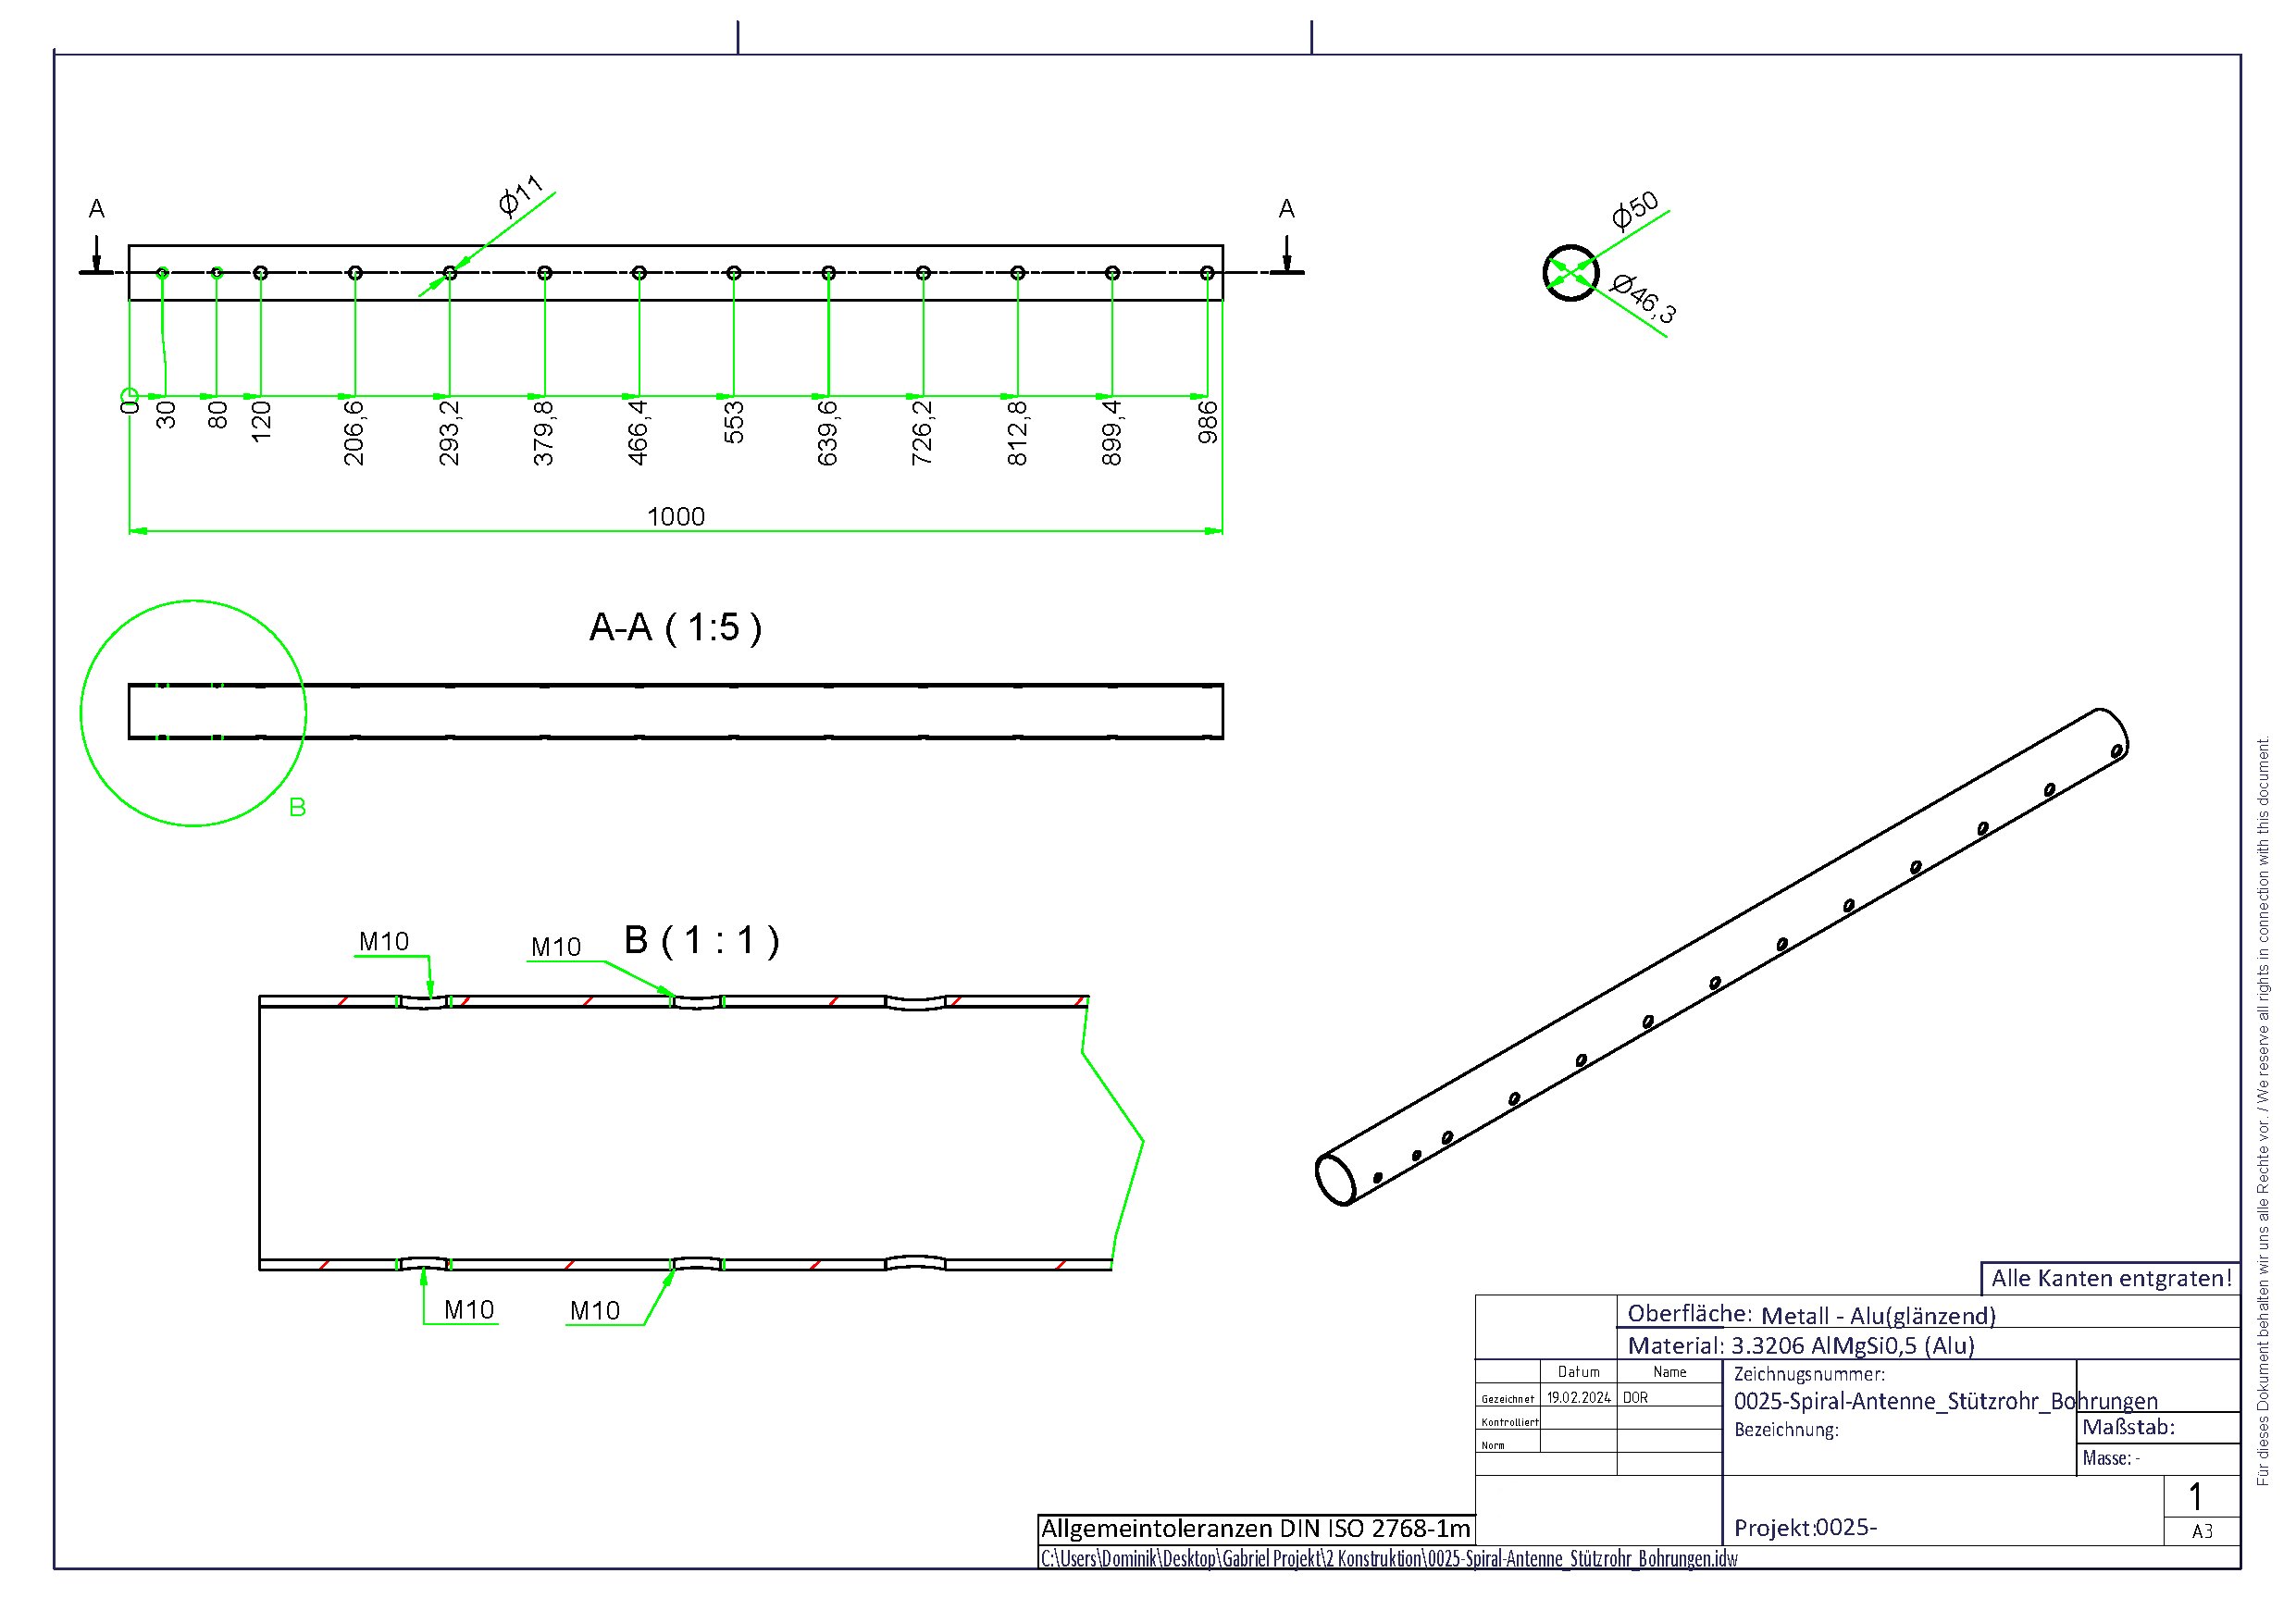
\includegraphics[width=\textwidth]{../ref/0025-Spiral-Antenne_St_tzrohr_Bohrungen.pdf}
	\caption{Der Bohrplan des PVC-Rohres}
	\label{fig:PVCU-Rohr-Bohrplan}
\end{figure}

Wie an der Zeichnung zu erkennen ist, wurden Löcher mit einem Abstand von 86,6mm und einem Durchmesser von 11mm gebohrt. Diese schaffen genug Platz für die Seitenelemente welche einen Durchmesser von 10mm aufweisen. Um das Rohr mithilfe des Rohrflansches an der Reflektorplatte zu montieren wurden zwei Löcher mit M10-Gewinde gebohrt. 

Das gewählte Material ist PTFE, da es eine sehr niedrige elektrische Permittivität besitzt. Das ist wichtig, da die Spirale, welche die Resonanzfrequenz der Helixantenne bestimmt, so gut wie möglich von kapazitiven Einflüssen geschützt sein sollte. Das $\epsilon\textsubscript{r}$ von PTFE ist rund 2,2, während das von Luft ca. 1 ist \cite{lipinski_polytetrafluorethylen_nodate,noauthor_dielektrizitatskonstante_nodate}. Teflon ist zwar ein relativ weicher Kunststoff, allerdings erhöht die Anordnung der Seitenelemente die strukturelle Stabilität der Konstruktion. Da PTFE UV-beständig ist, eignet dieser sich bestens für den Einsatz im Freien.

\begin{figure}[h!]
	\centering
	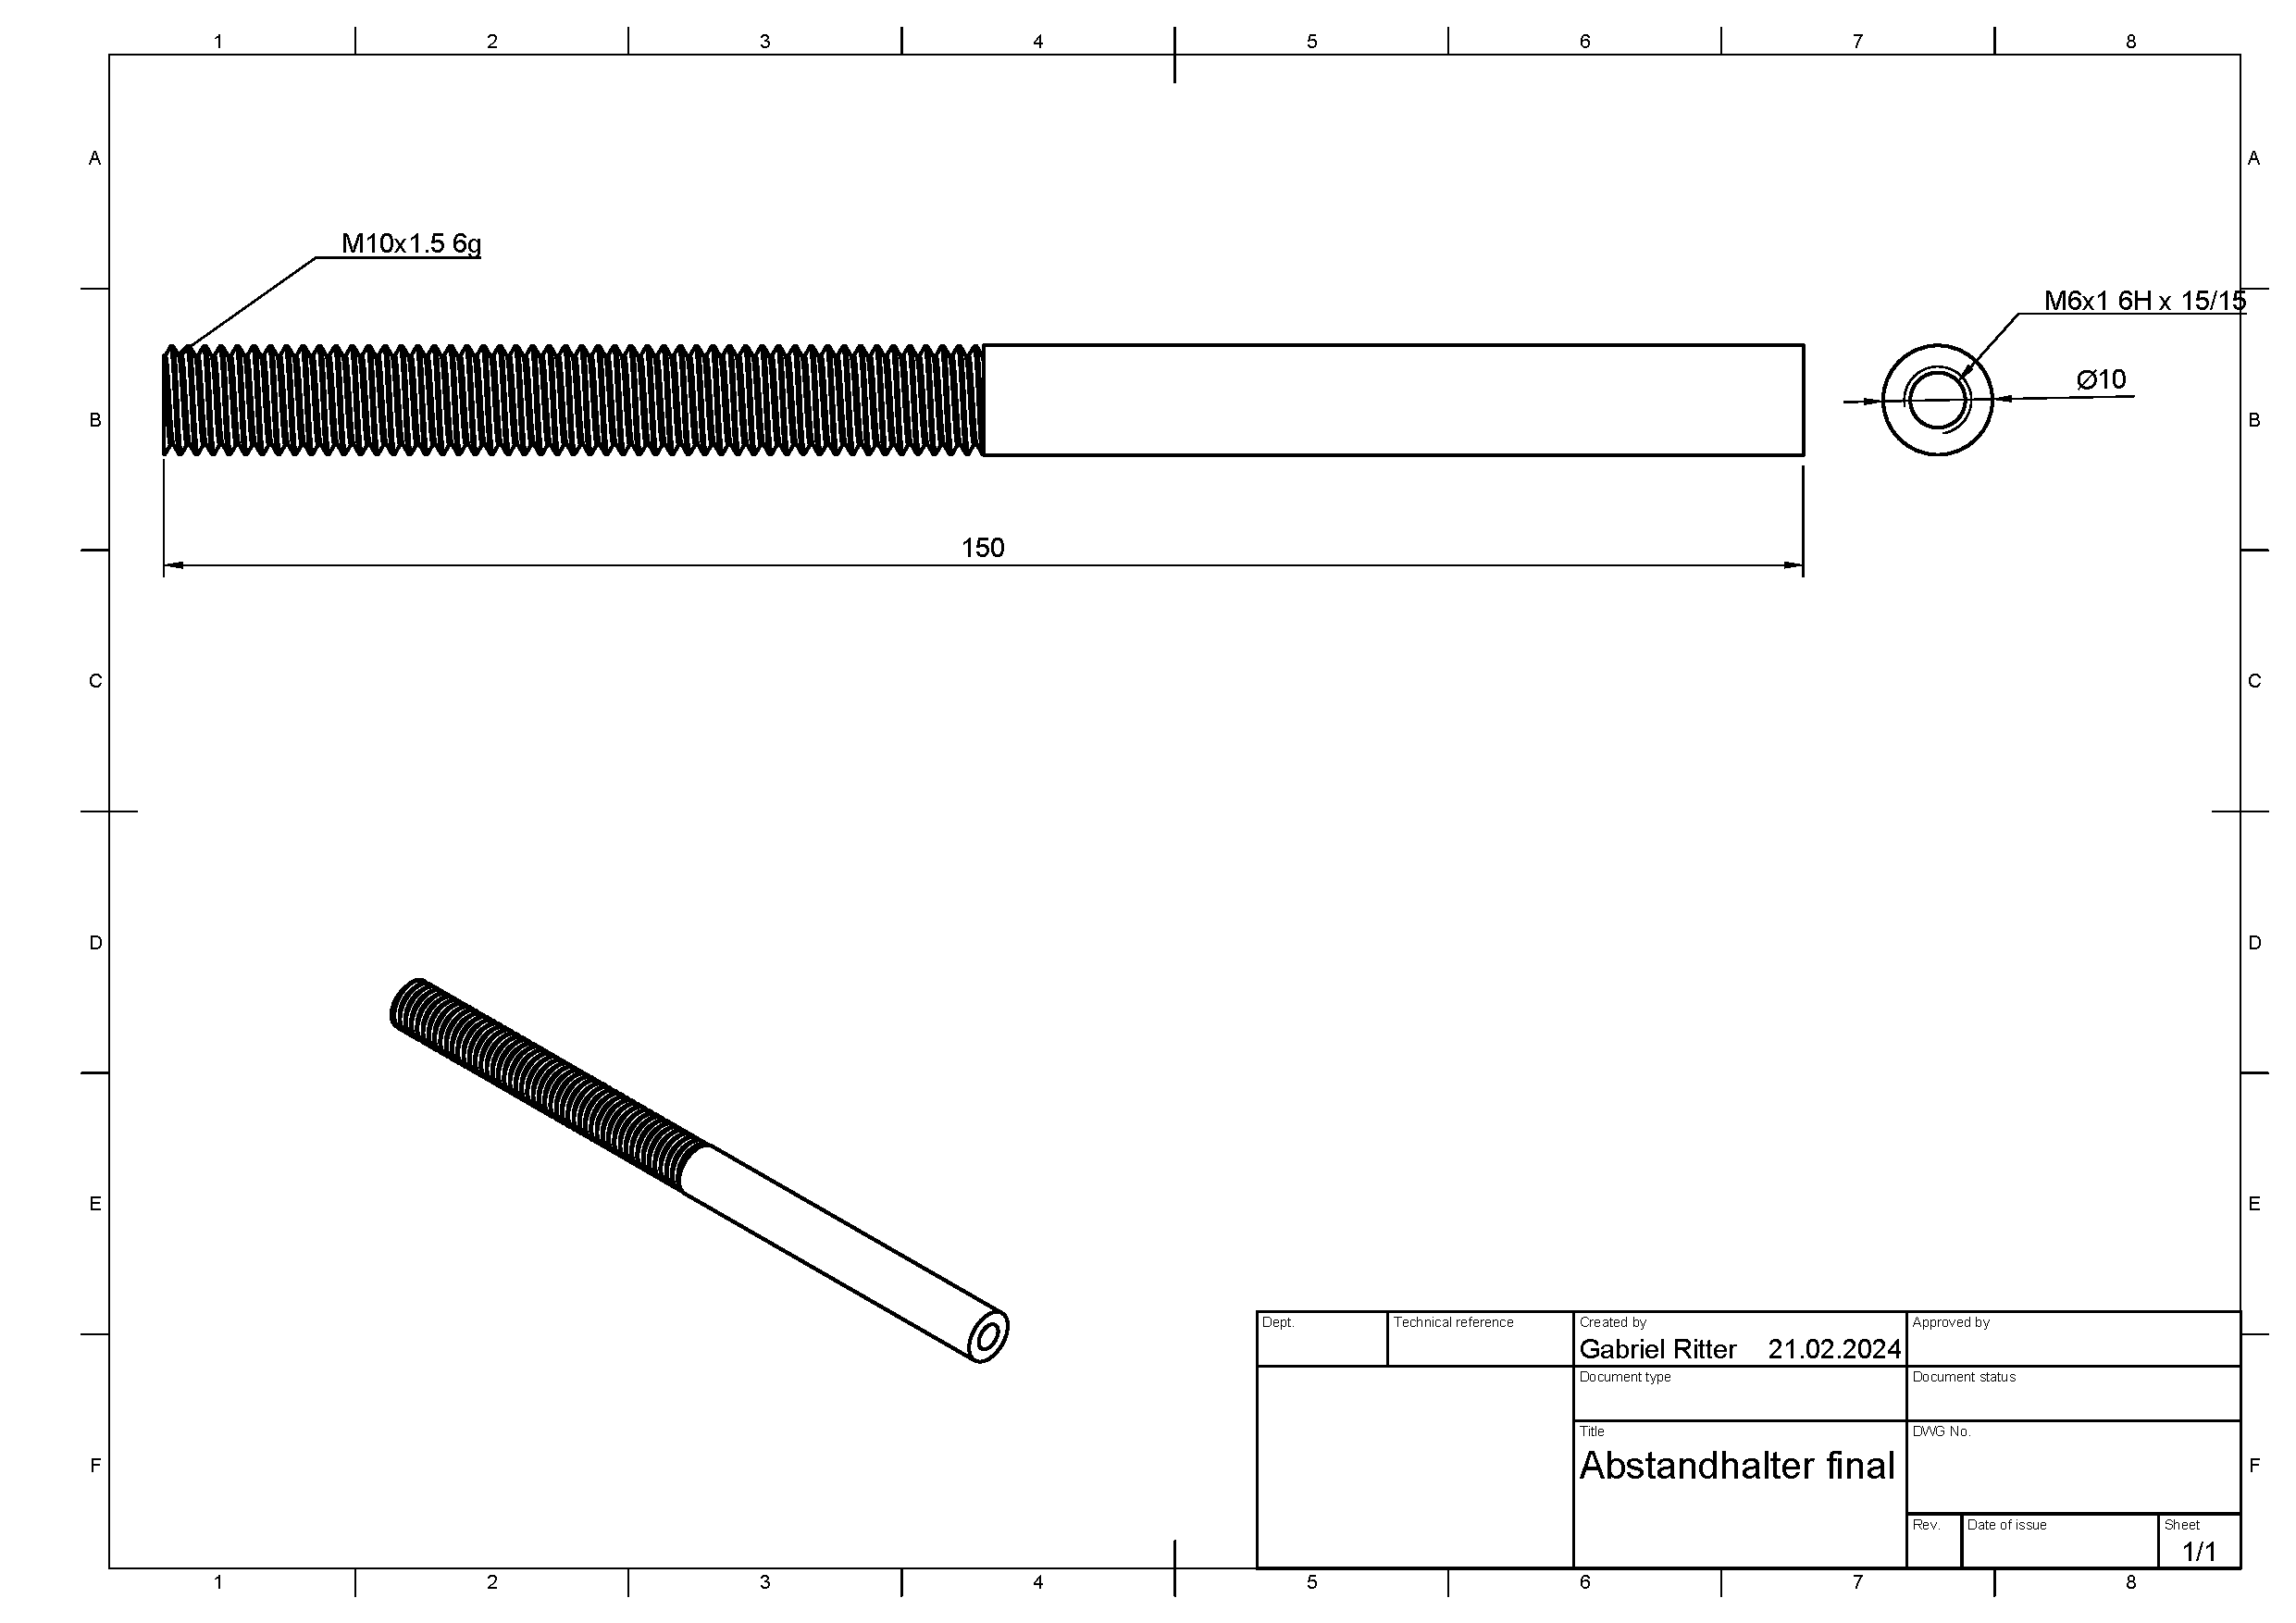
\includegraphics[width=\textwidth]{../ref/Abstandhalter final Zeichnung v2.pdf}
	\caption{Zeichnung des Abstandhalters}
	\label{fig:Abstandhalter-Zeichnung}
\end{figure}

\begin{figure}[h!]
	\centering
	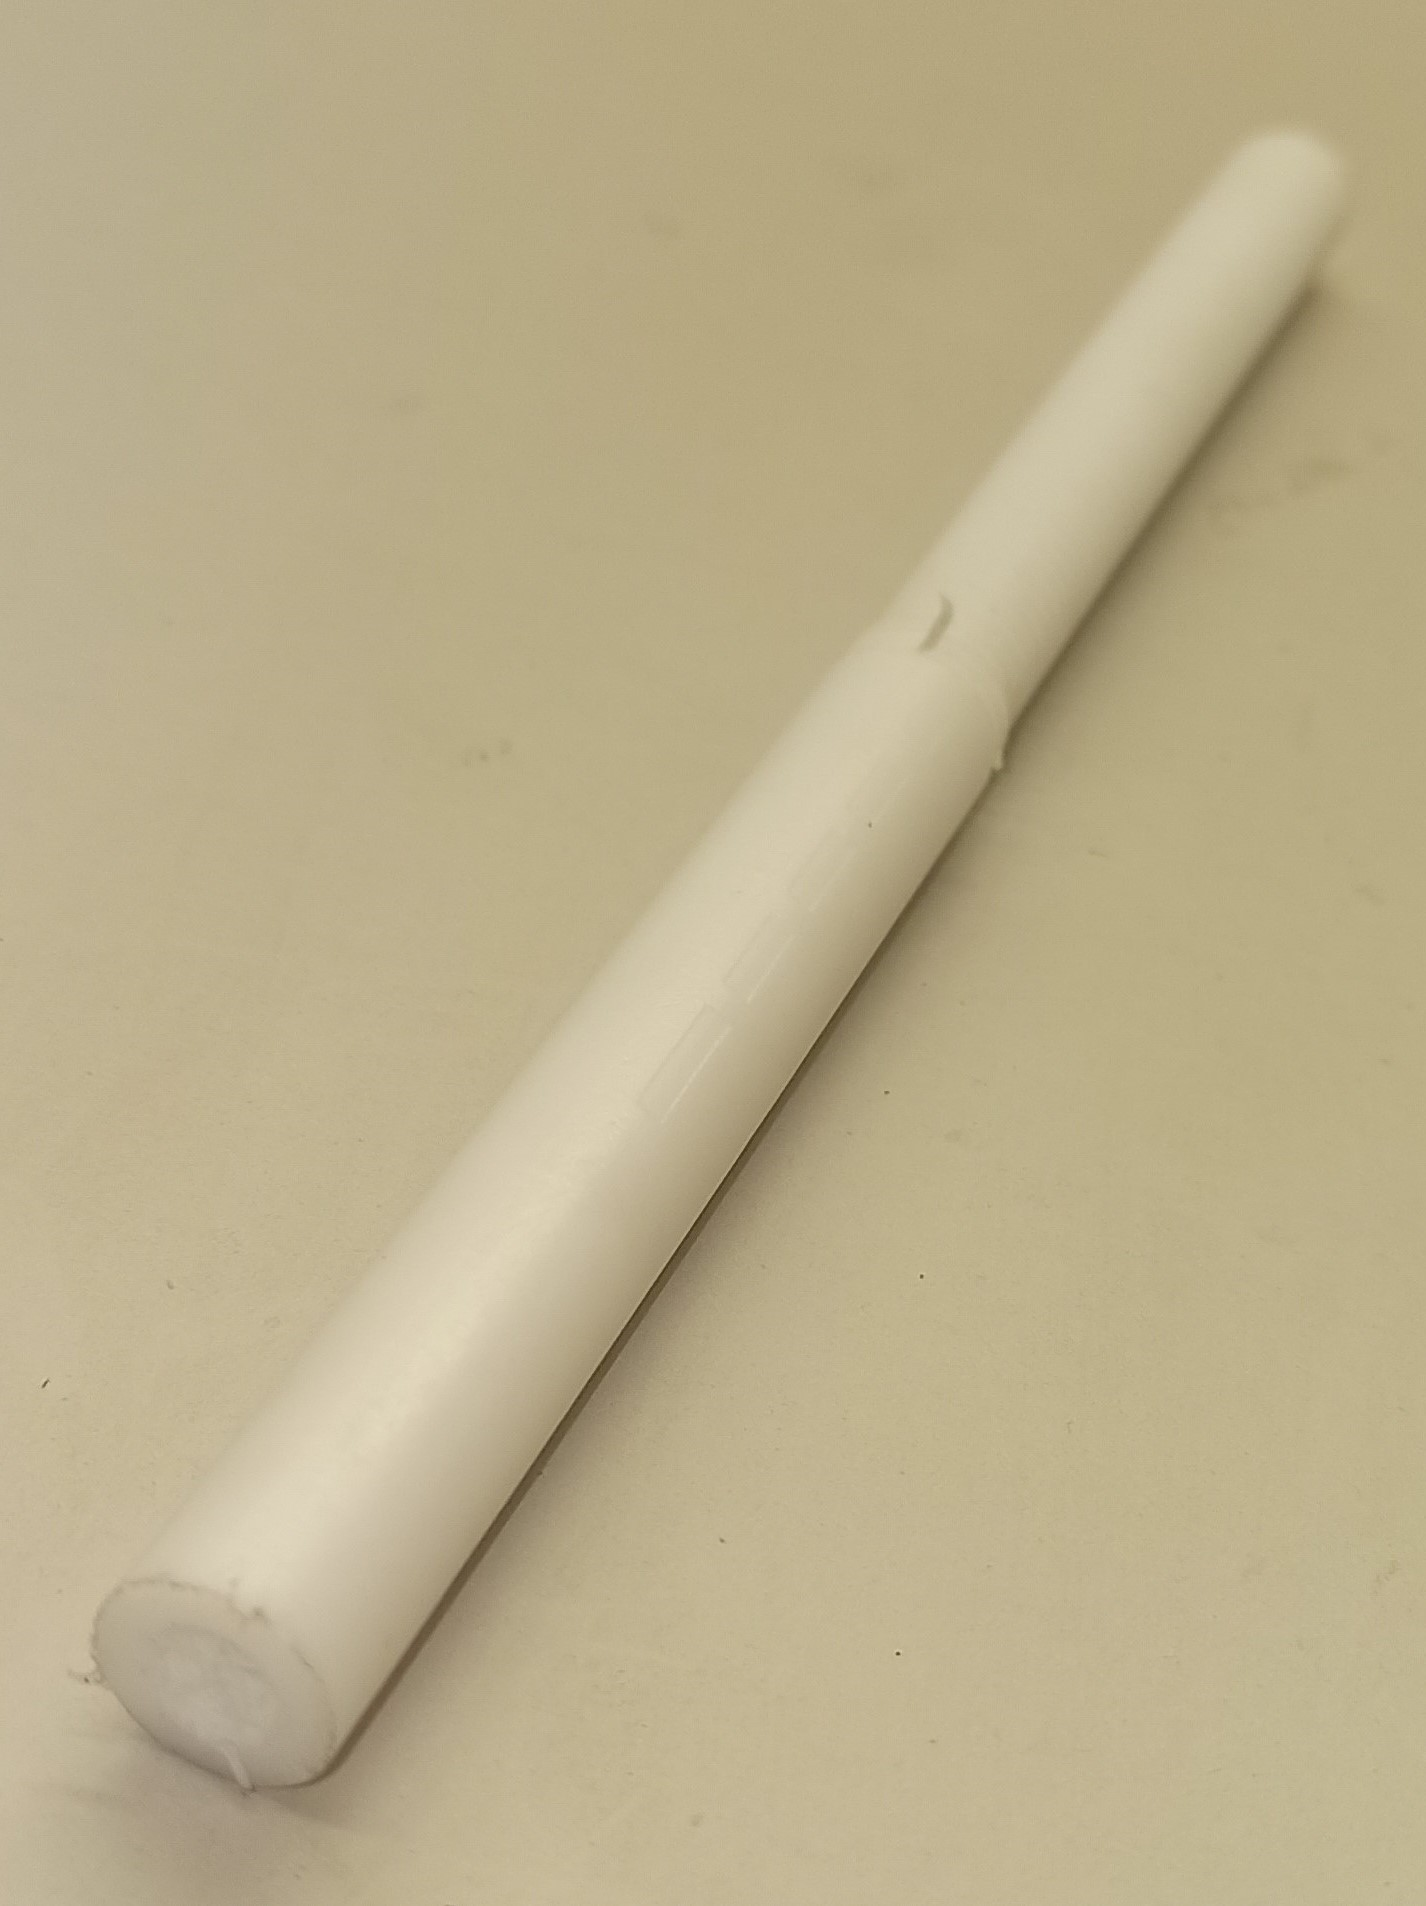
\includegraphics[width=\textwidth]{../ref/Abstandhalter-real.jpg}
	\caption{Realer Abstandhalter}
	\label{fig:Abstandhalter-real}
\end{figure}

An der Zeichnung sowie an dem realen Bauteil lässt sich erkennen, dass das Außengewinde ungefähr bis zur Mitte der Teflonstange geschnitten ist. Der Stab wird mit dem Gewinde zuerst in die Löcher des PVC-Rohres gesteckt, damit dieser von vorne und hinten mit M10-Kunststoffmuttern an das Rohr geschraubt werden kann.

%BILD MUSS NOCH GEÄNDERT WERDEN (Bild der Befestigung)
\begin{figure}[h!]
	\centering
	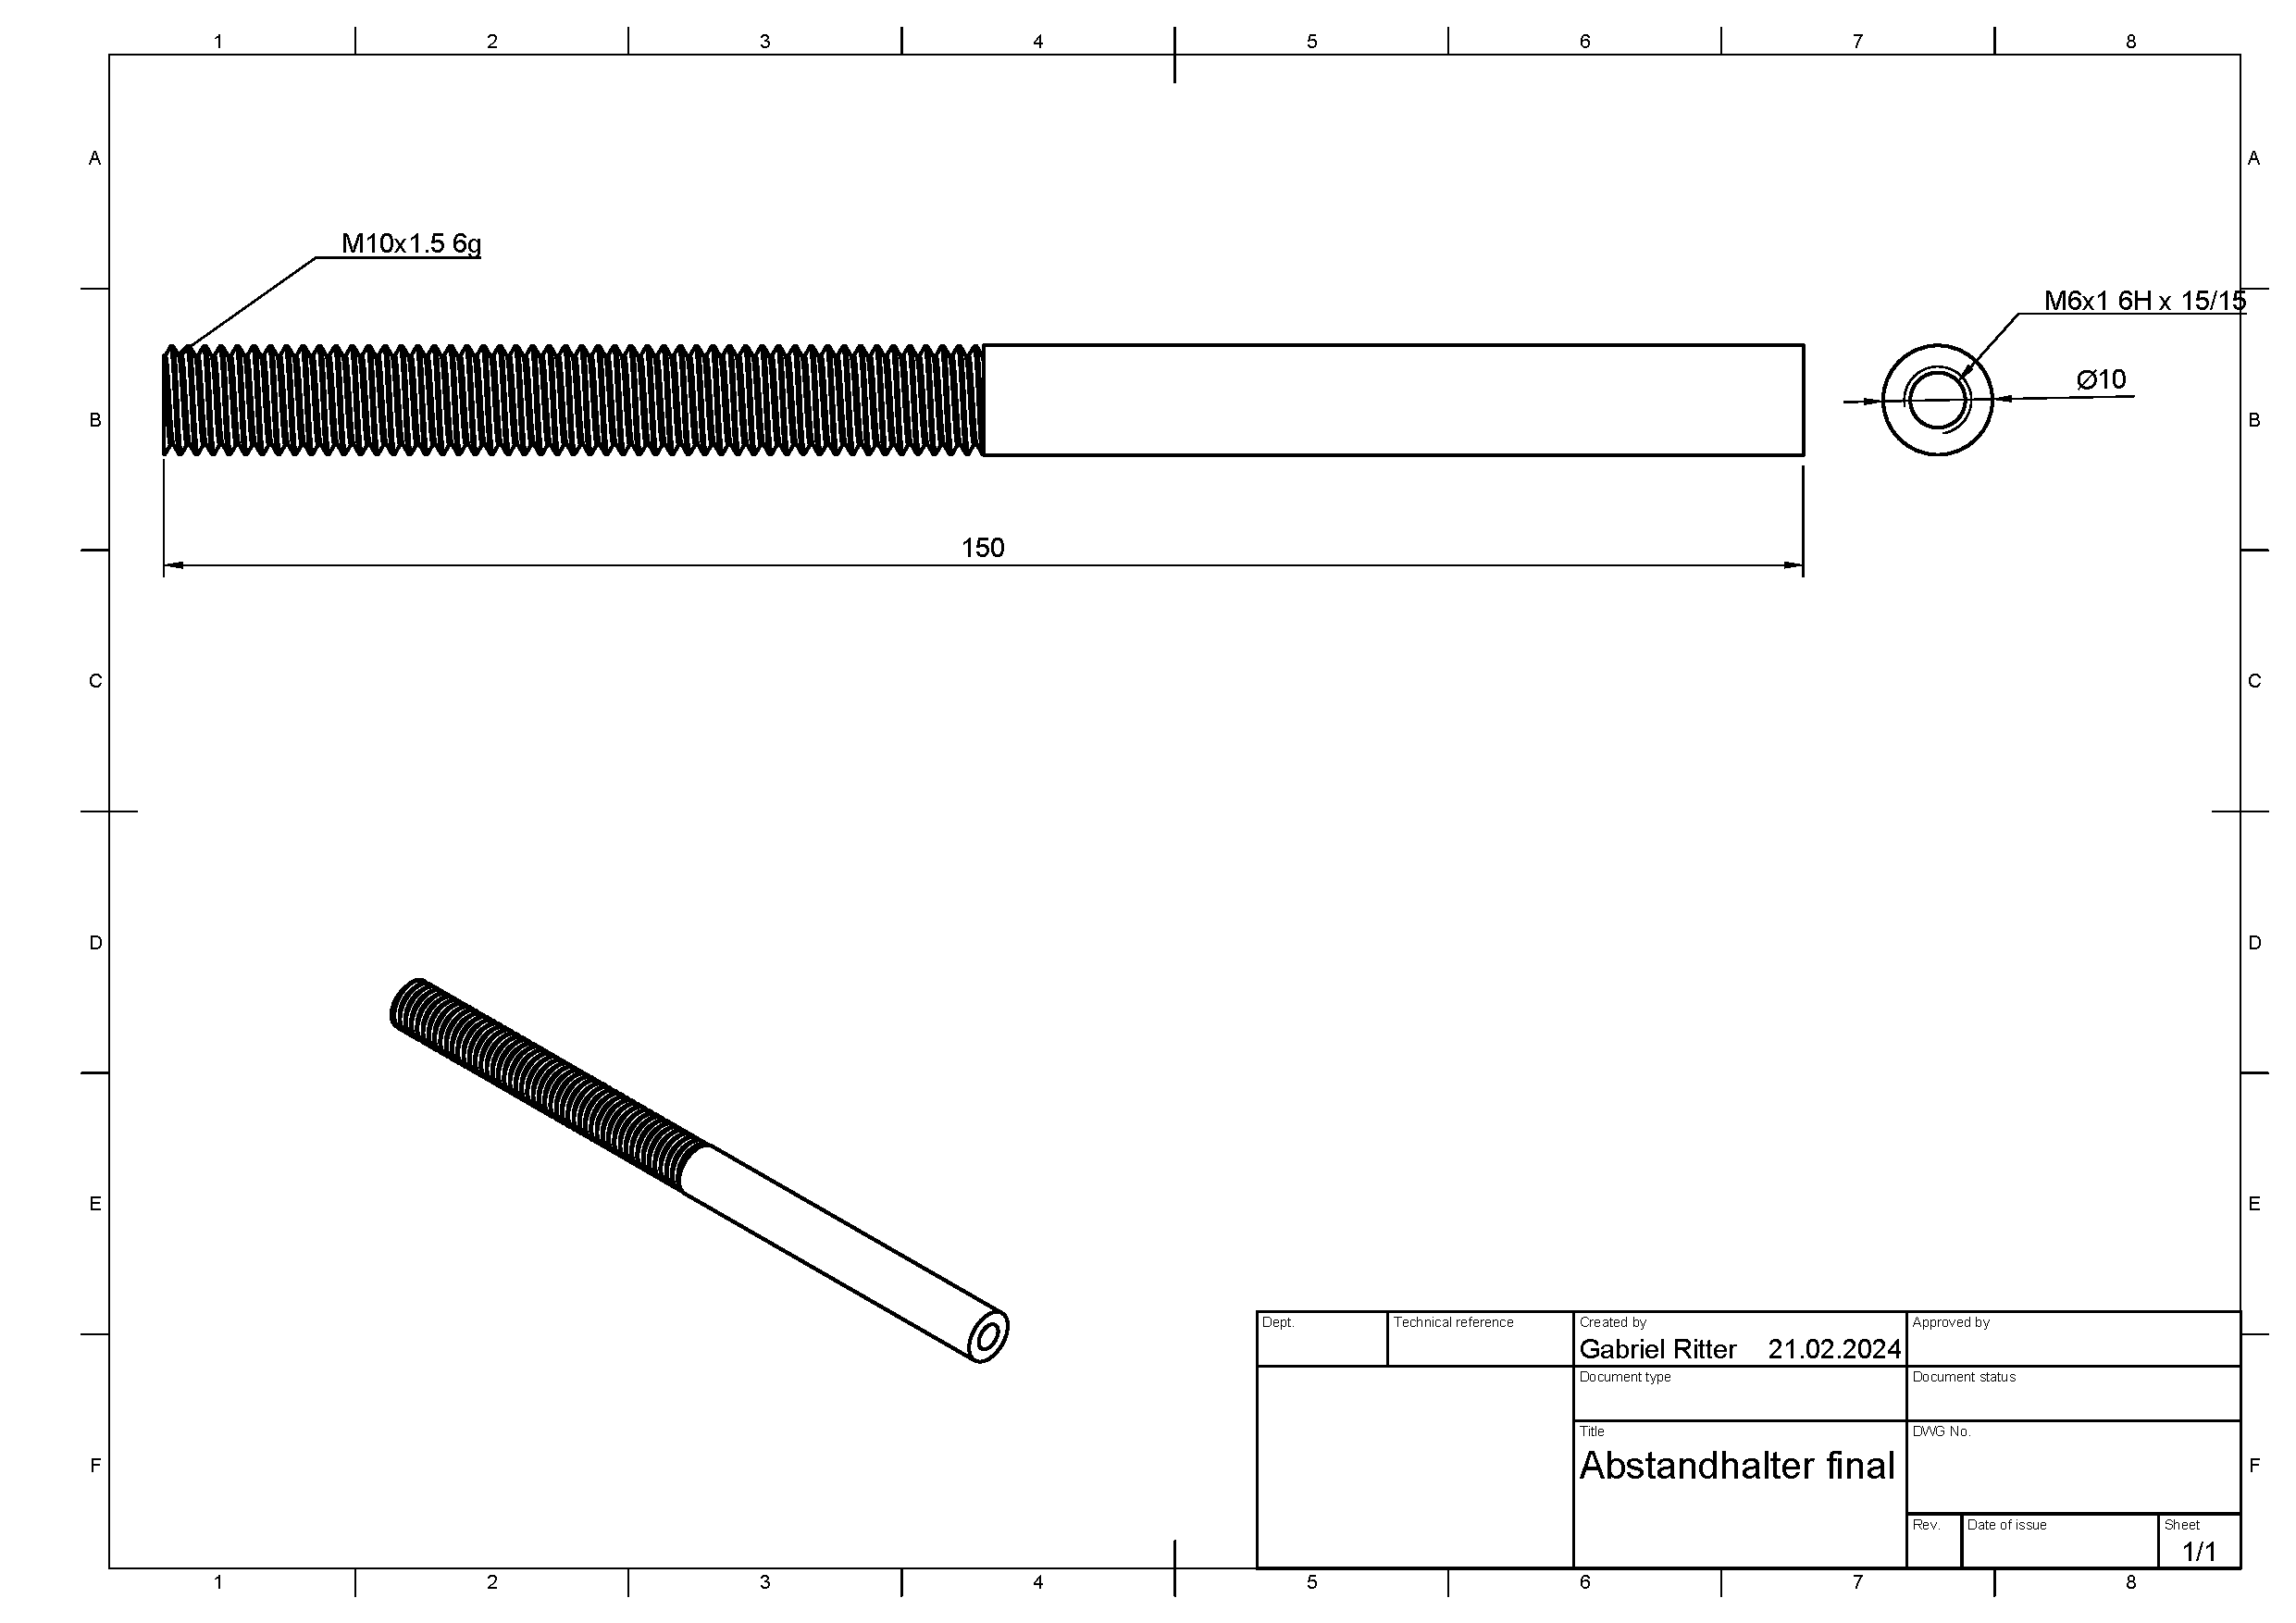
\includegraphics[width=\textwidth]{../ref/Abstandhalter final Zeichnung v2.pdf}
	\caption{Befestigung der Abstandhalter am PVC-Rohr}
	\label{fig:Abstandhalter-Befestigung}
\end{figure}

In die gegenüberliegende Seite des Außengewindes wird ein Loch mit einem Durchmesser von 5mm für ein M6-Gewinde gebohrt. Mithilfe der entsprechenden Schrauben werden UV-stabilisierte Rohrschellen an dem Seitenelement montiert. Diese tolerieren Rohrdurchmesser von bis zu 18mm. Durch die Verwendung von Rohrschellen vereinfacht sich die Montage der Spirale auf ein einfaches Einschnappen des Rohres.

%Korrektes Bild fehlt
\begin{figure}[h!]
	\centering
	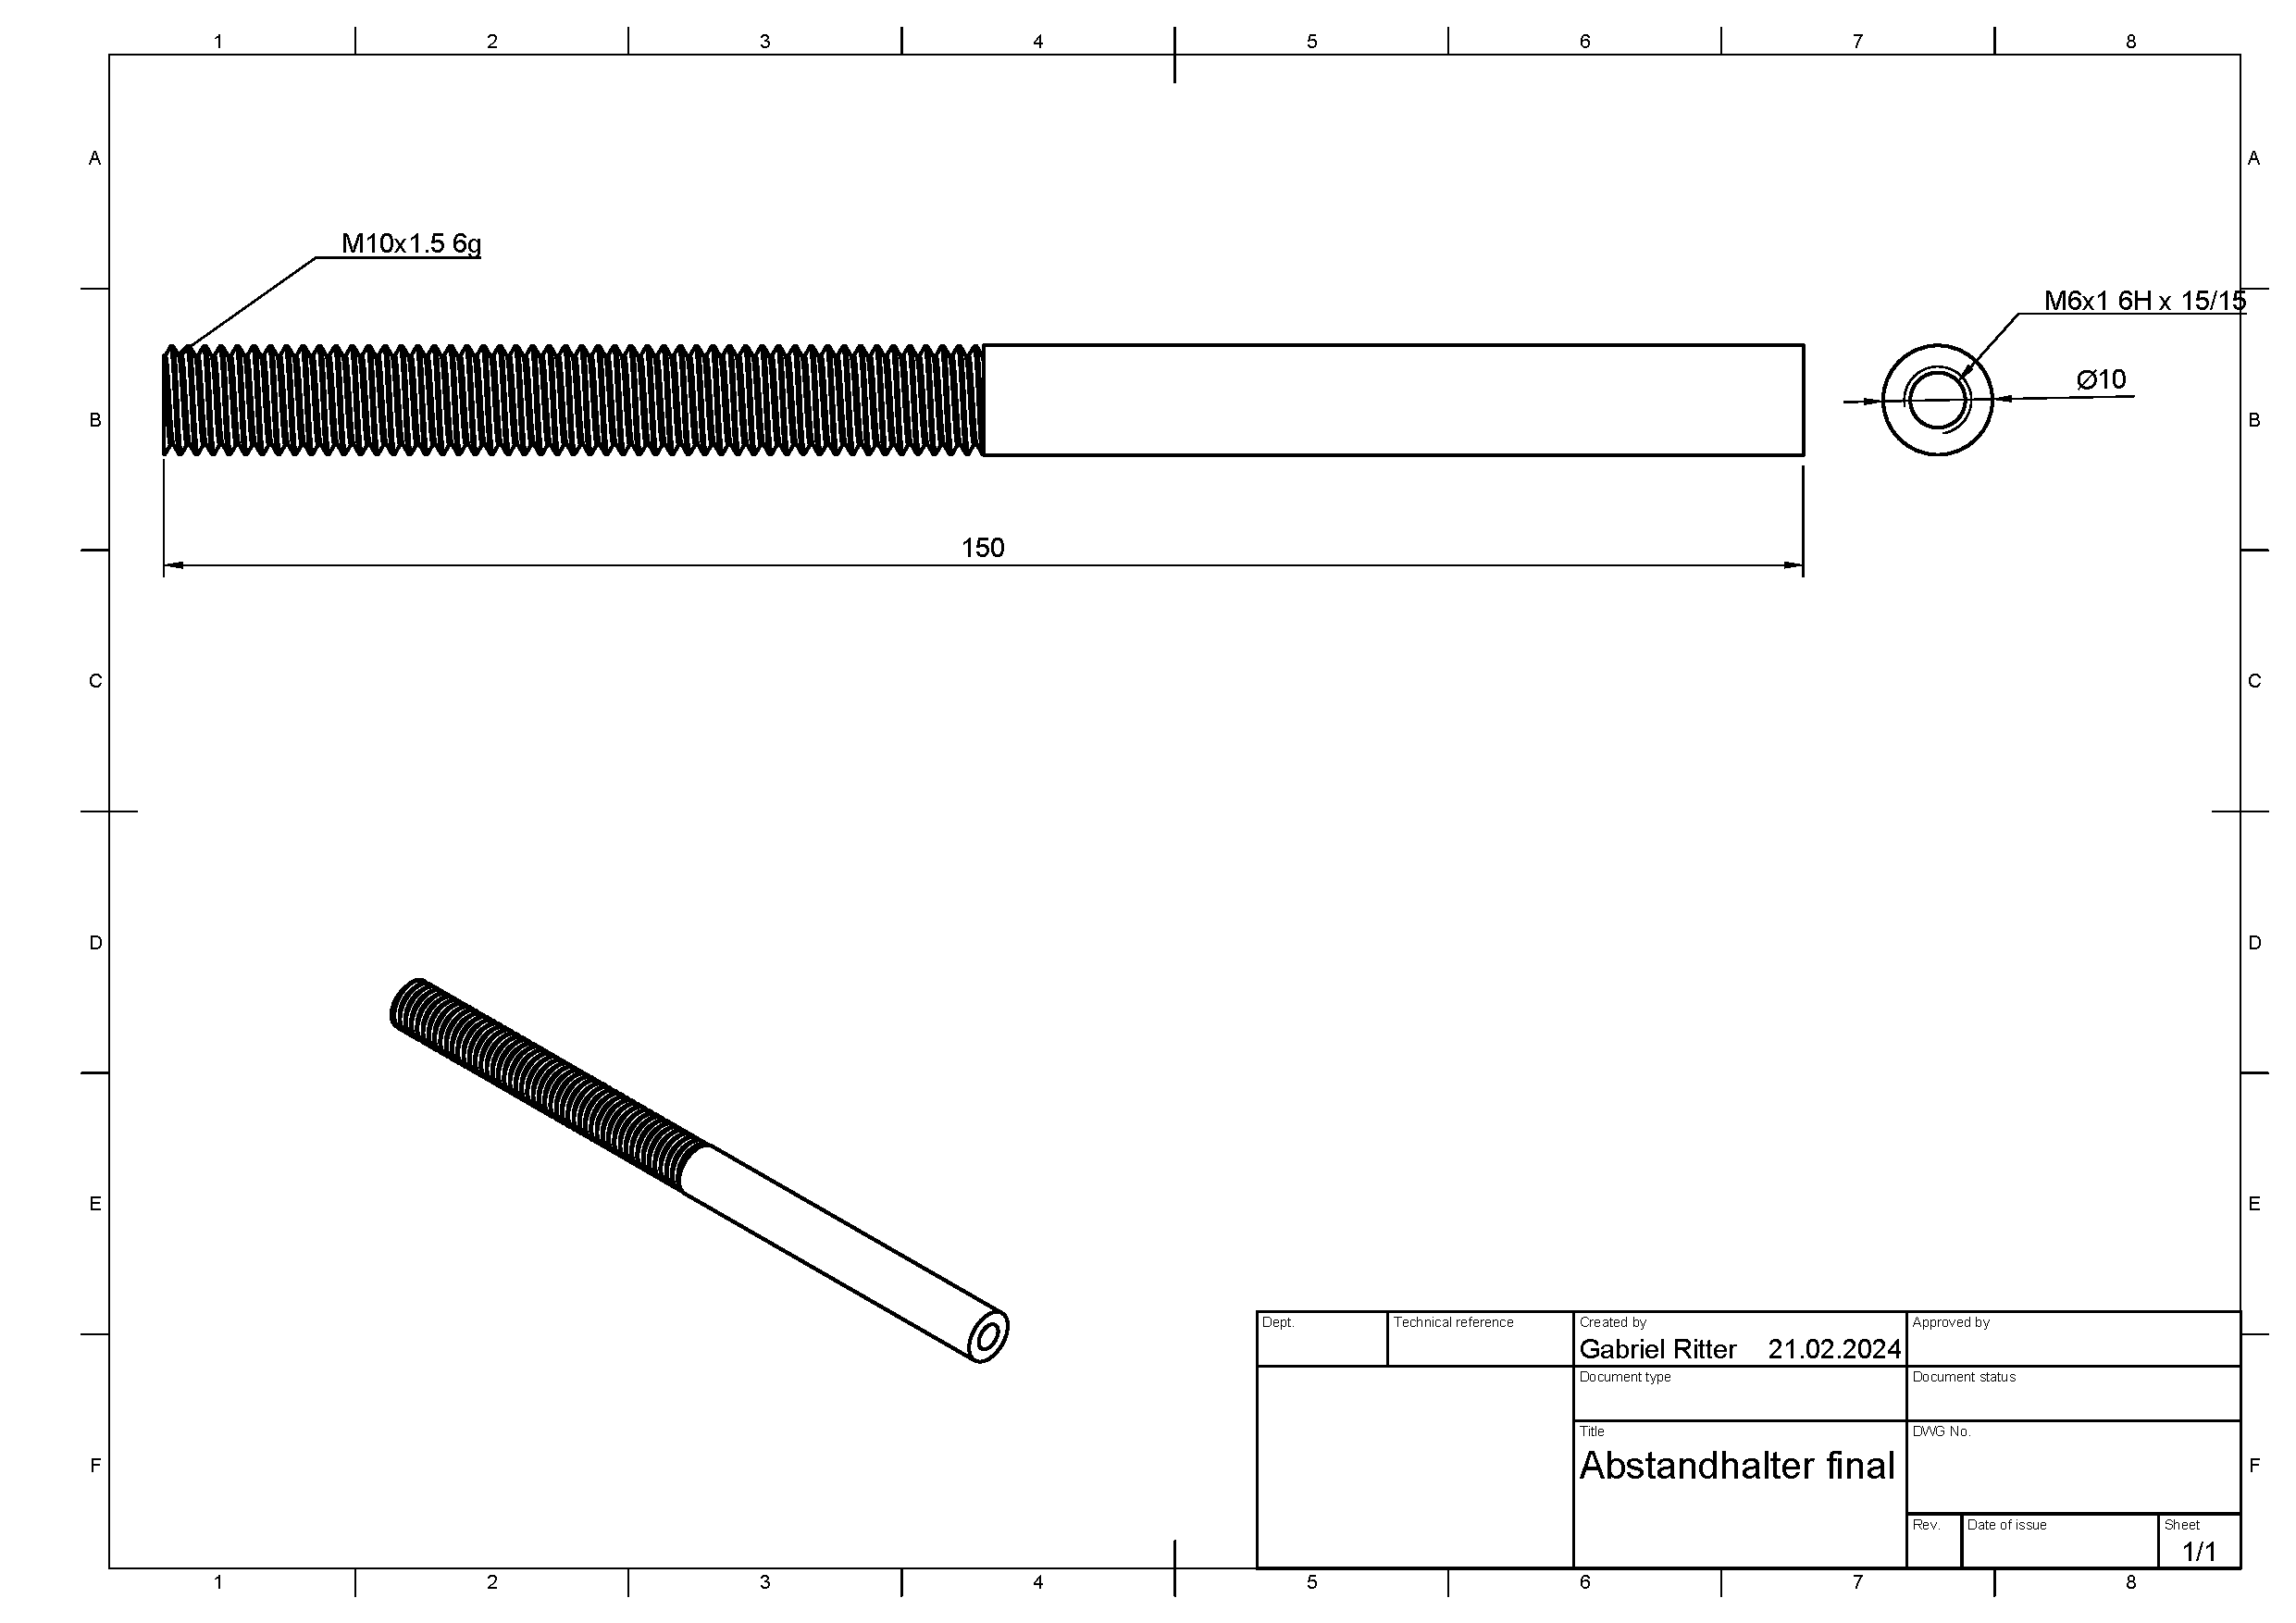
\includegraphics[width=\textwidth]{../ref/Abstandhalter final Zeichnung v2.pdf}
	\caption{Zusammengefügtes Seitenelement}
	\label{fig:Seitenelement-komplett}
\end{figure}

Der Rohrflansch bildet das Bindeelement zwischen dem PVC-Rohr und der Reflektorplatte. Dieser hat einen Innendurchmesser von 51mm, und eine Wandstärke von 4mm. Dadurch wird genug Toleranz geboten damit das PVC-Rohr sicher verschraubt werden kann. 

\begin{figure}[h!]
	\centering
	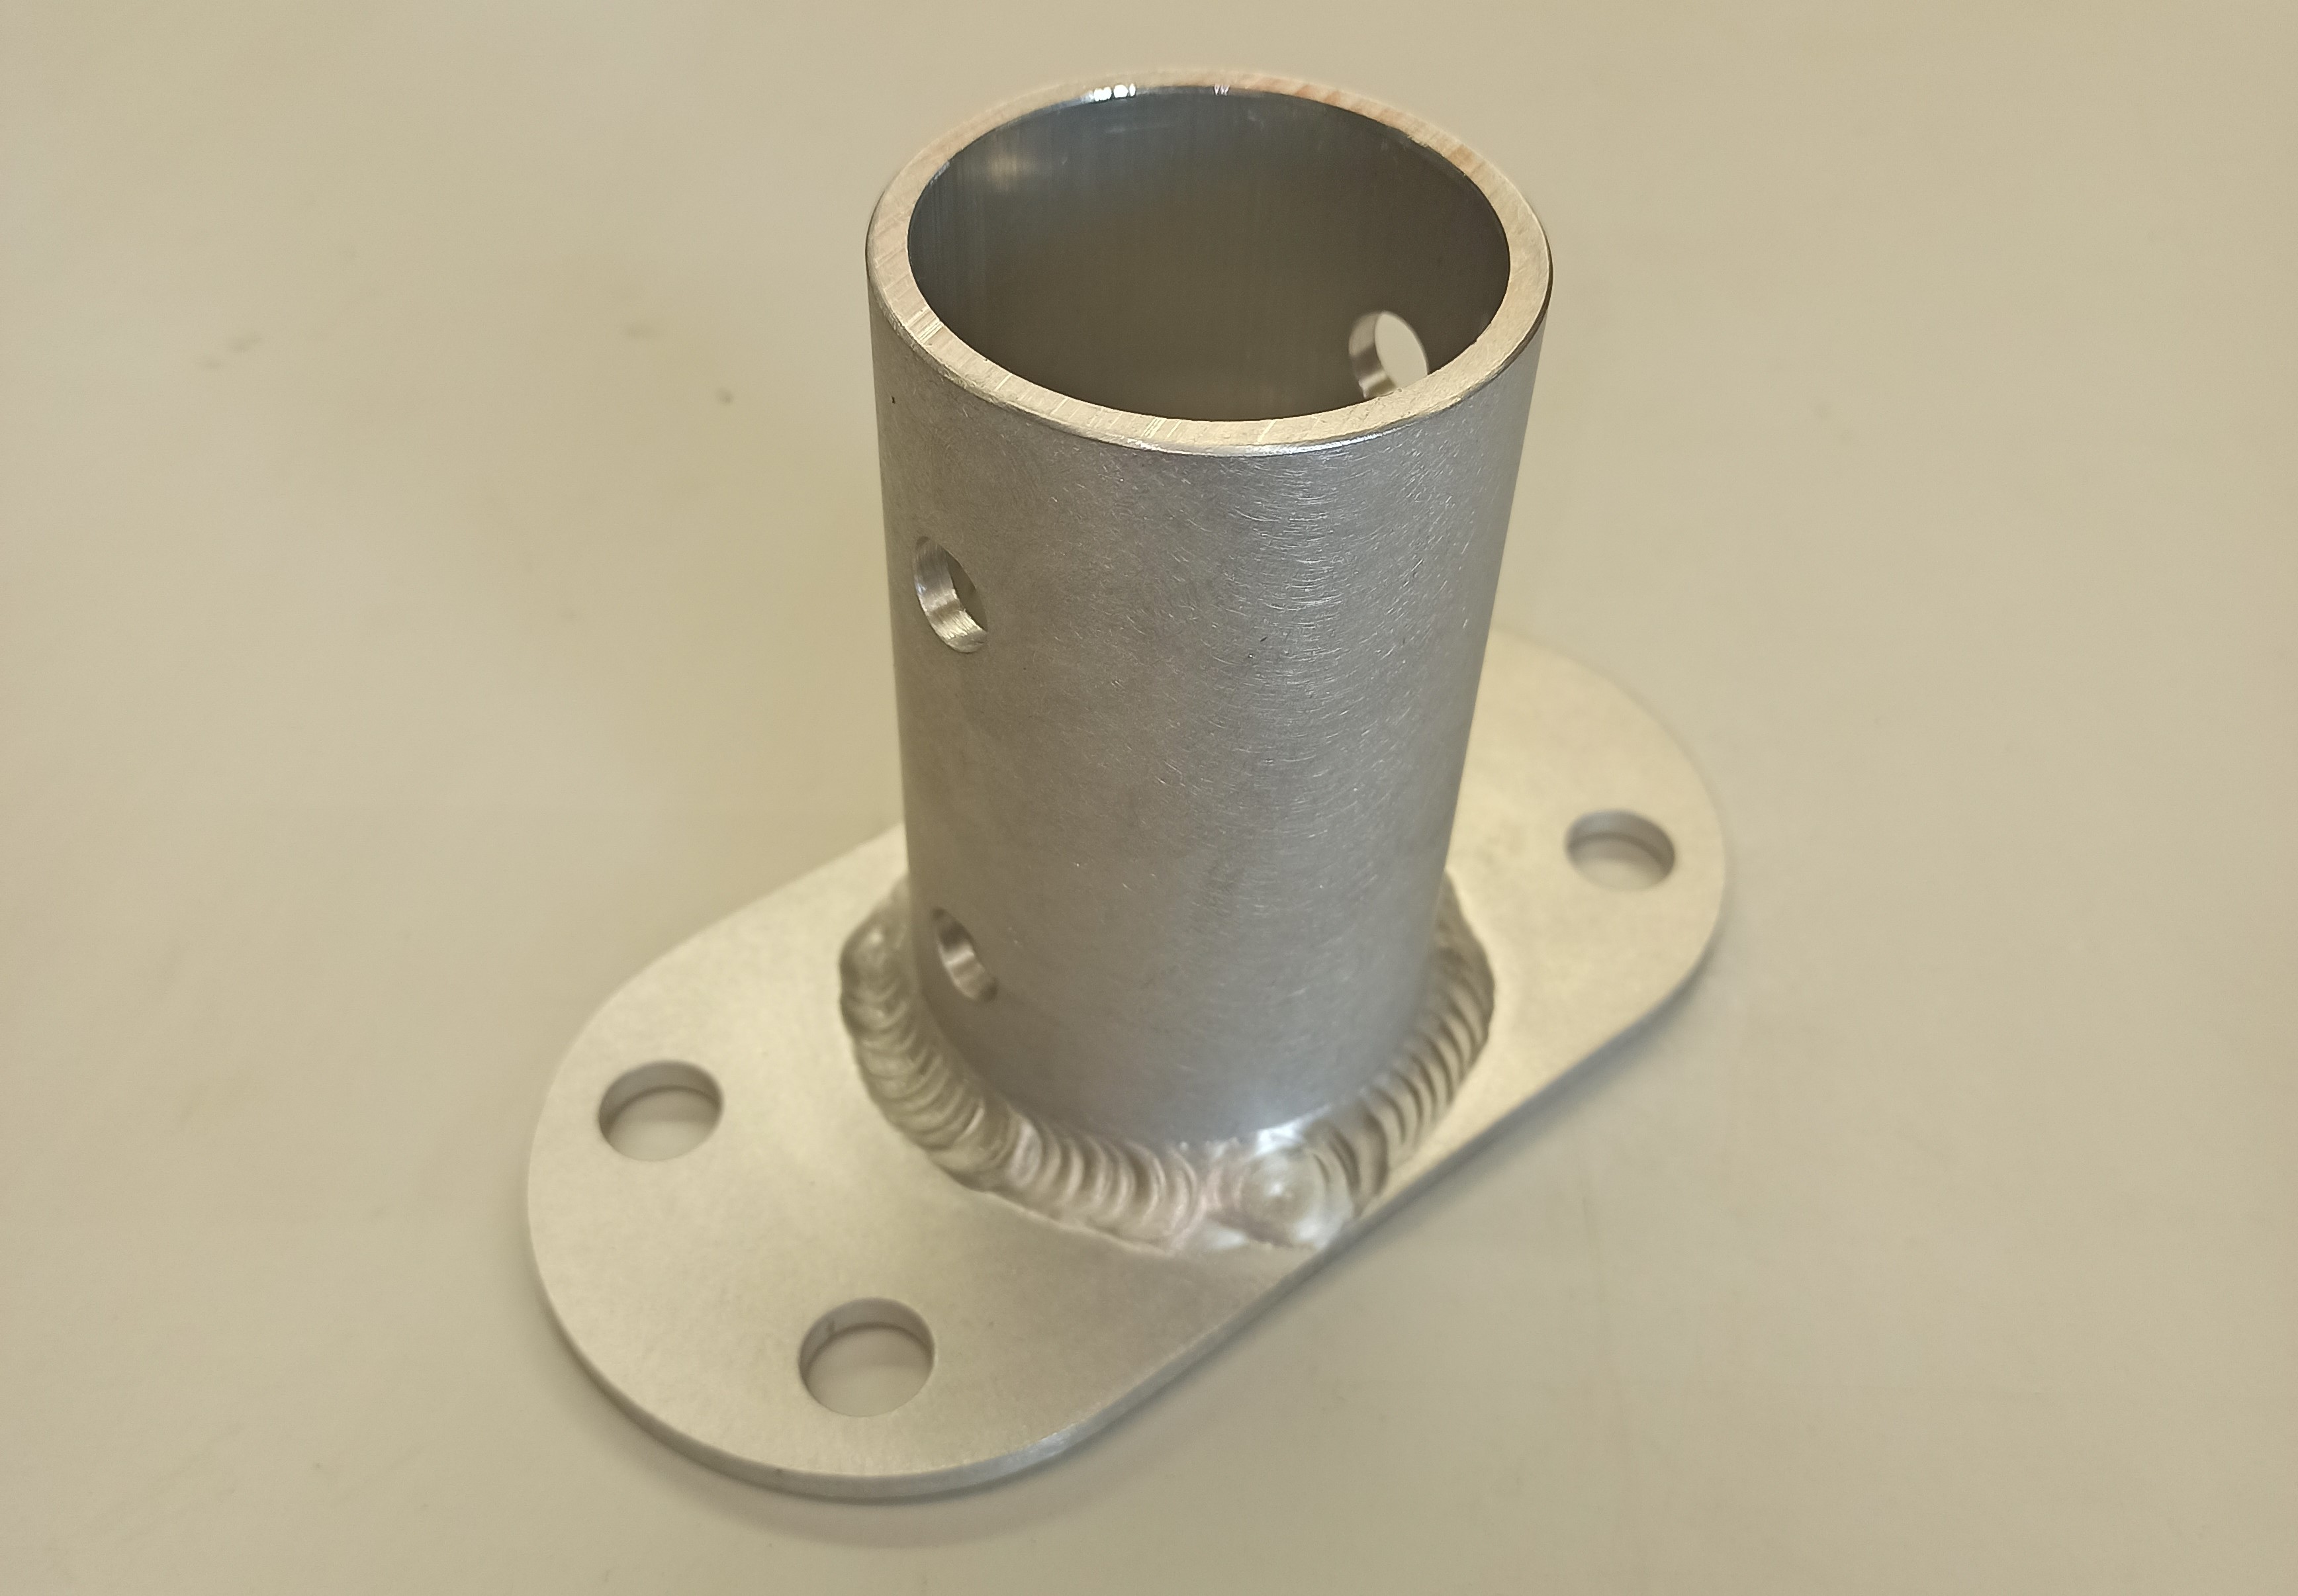
\includegraphics[width=\textwidth]{../ref/Antenne-Rohrflansch.jpg}
	\caption{Rohrflansch zur Befestigung des PVC-Rohres}
	\label{fig:Rohrflansch-Antenne}
\end{figure}

Der Rohrflansch besteht aus einem Rohr, in welches zwei durchgehende Löcher mit einem Durchmesser von 11mm gebohrt wurden, und einer Platte in die ebenfalls zwei Löcher mit einem Durchmesser von 13,5mm gebohrt wurden. Die Platte und das Rohr werden aneinander geschweißt. Das resultierende Bauteil bildet das Bindeglied zwischen Reflektor und PVC-Rohr.

%Korrektes Bild fehlt (Verbindung zwischen Rohrflansch und Reflektor)
\begin{figure}[h!]
	\centering
	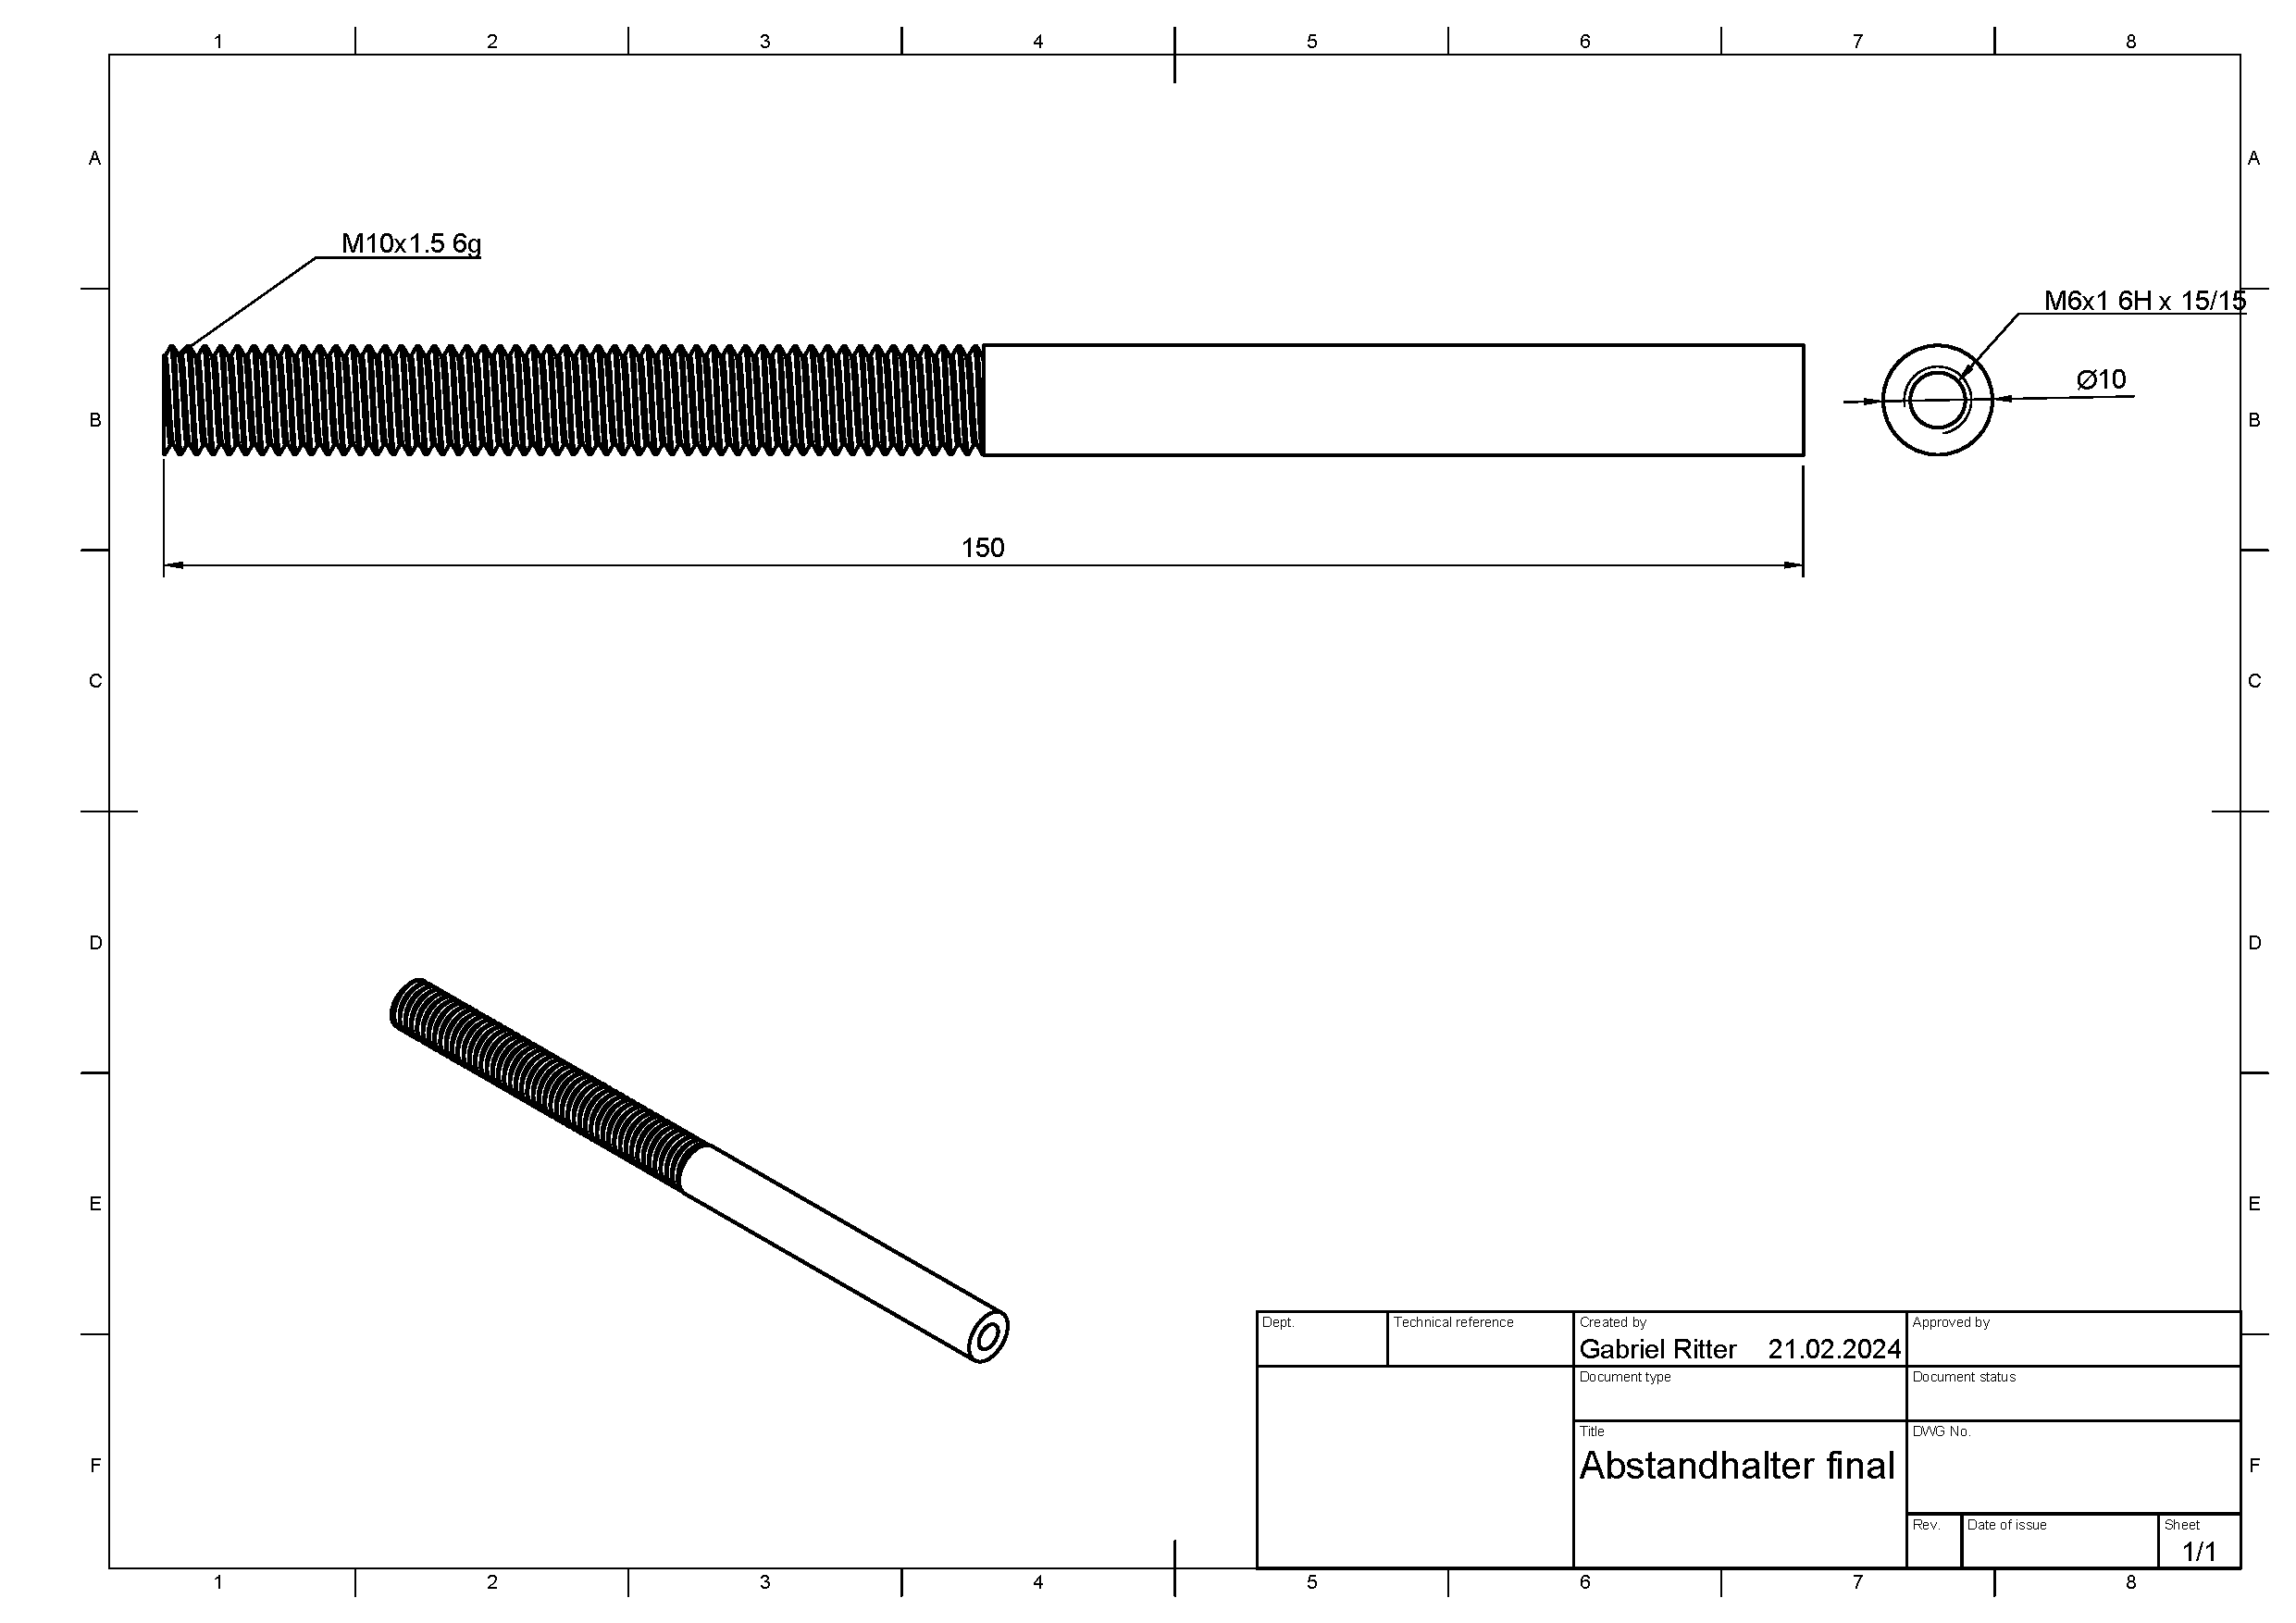
\includegraphics[width=\textwidth]{../ref/Abstandhalter final Zeichnung v2.pdf}
	\caption{Befestigung des Rohrflansches}
	\label{fig:Rohrflansch-Antenne-Verbindung}
\end{figure}

%NOCH UMZUFORMULIEREN
Für den Reflektor wurde eine runde Aluminiumplatte gewählt. Für die reale Konstruktion wurden Löcher in den äußeren Rand der Platte gelasert, um den Luftwiderstand zu reduzieren. Diese sollten kleiner als $\frac{\lambda}{7}$ sein, um unerwünschte Störungen zu vermeiden.

\begin{figure}[h!]
	\centering
	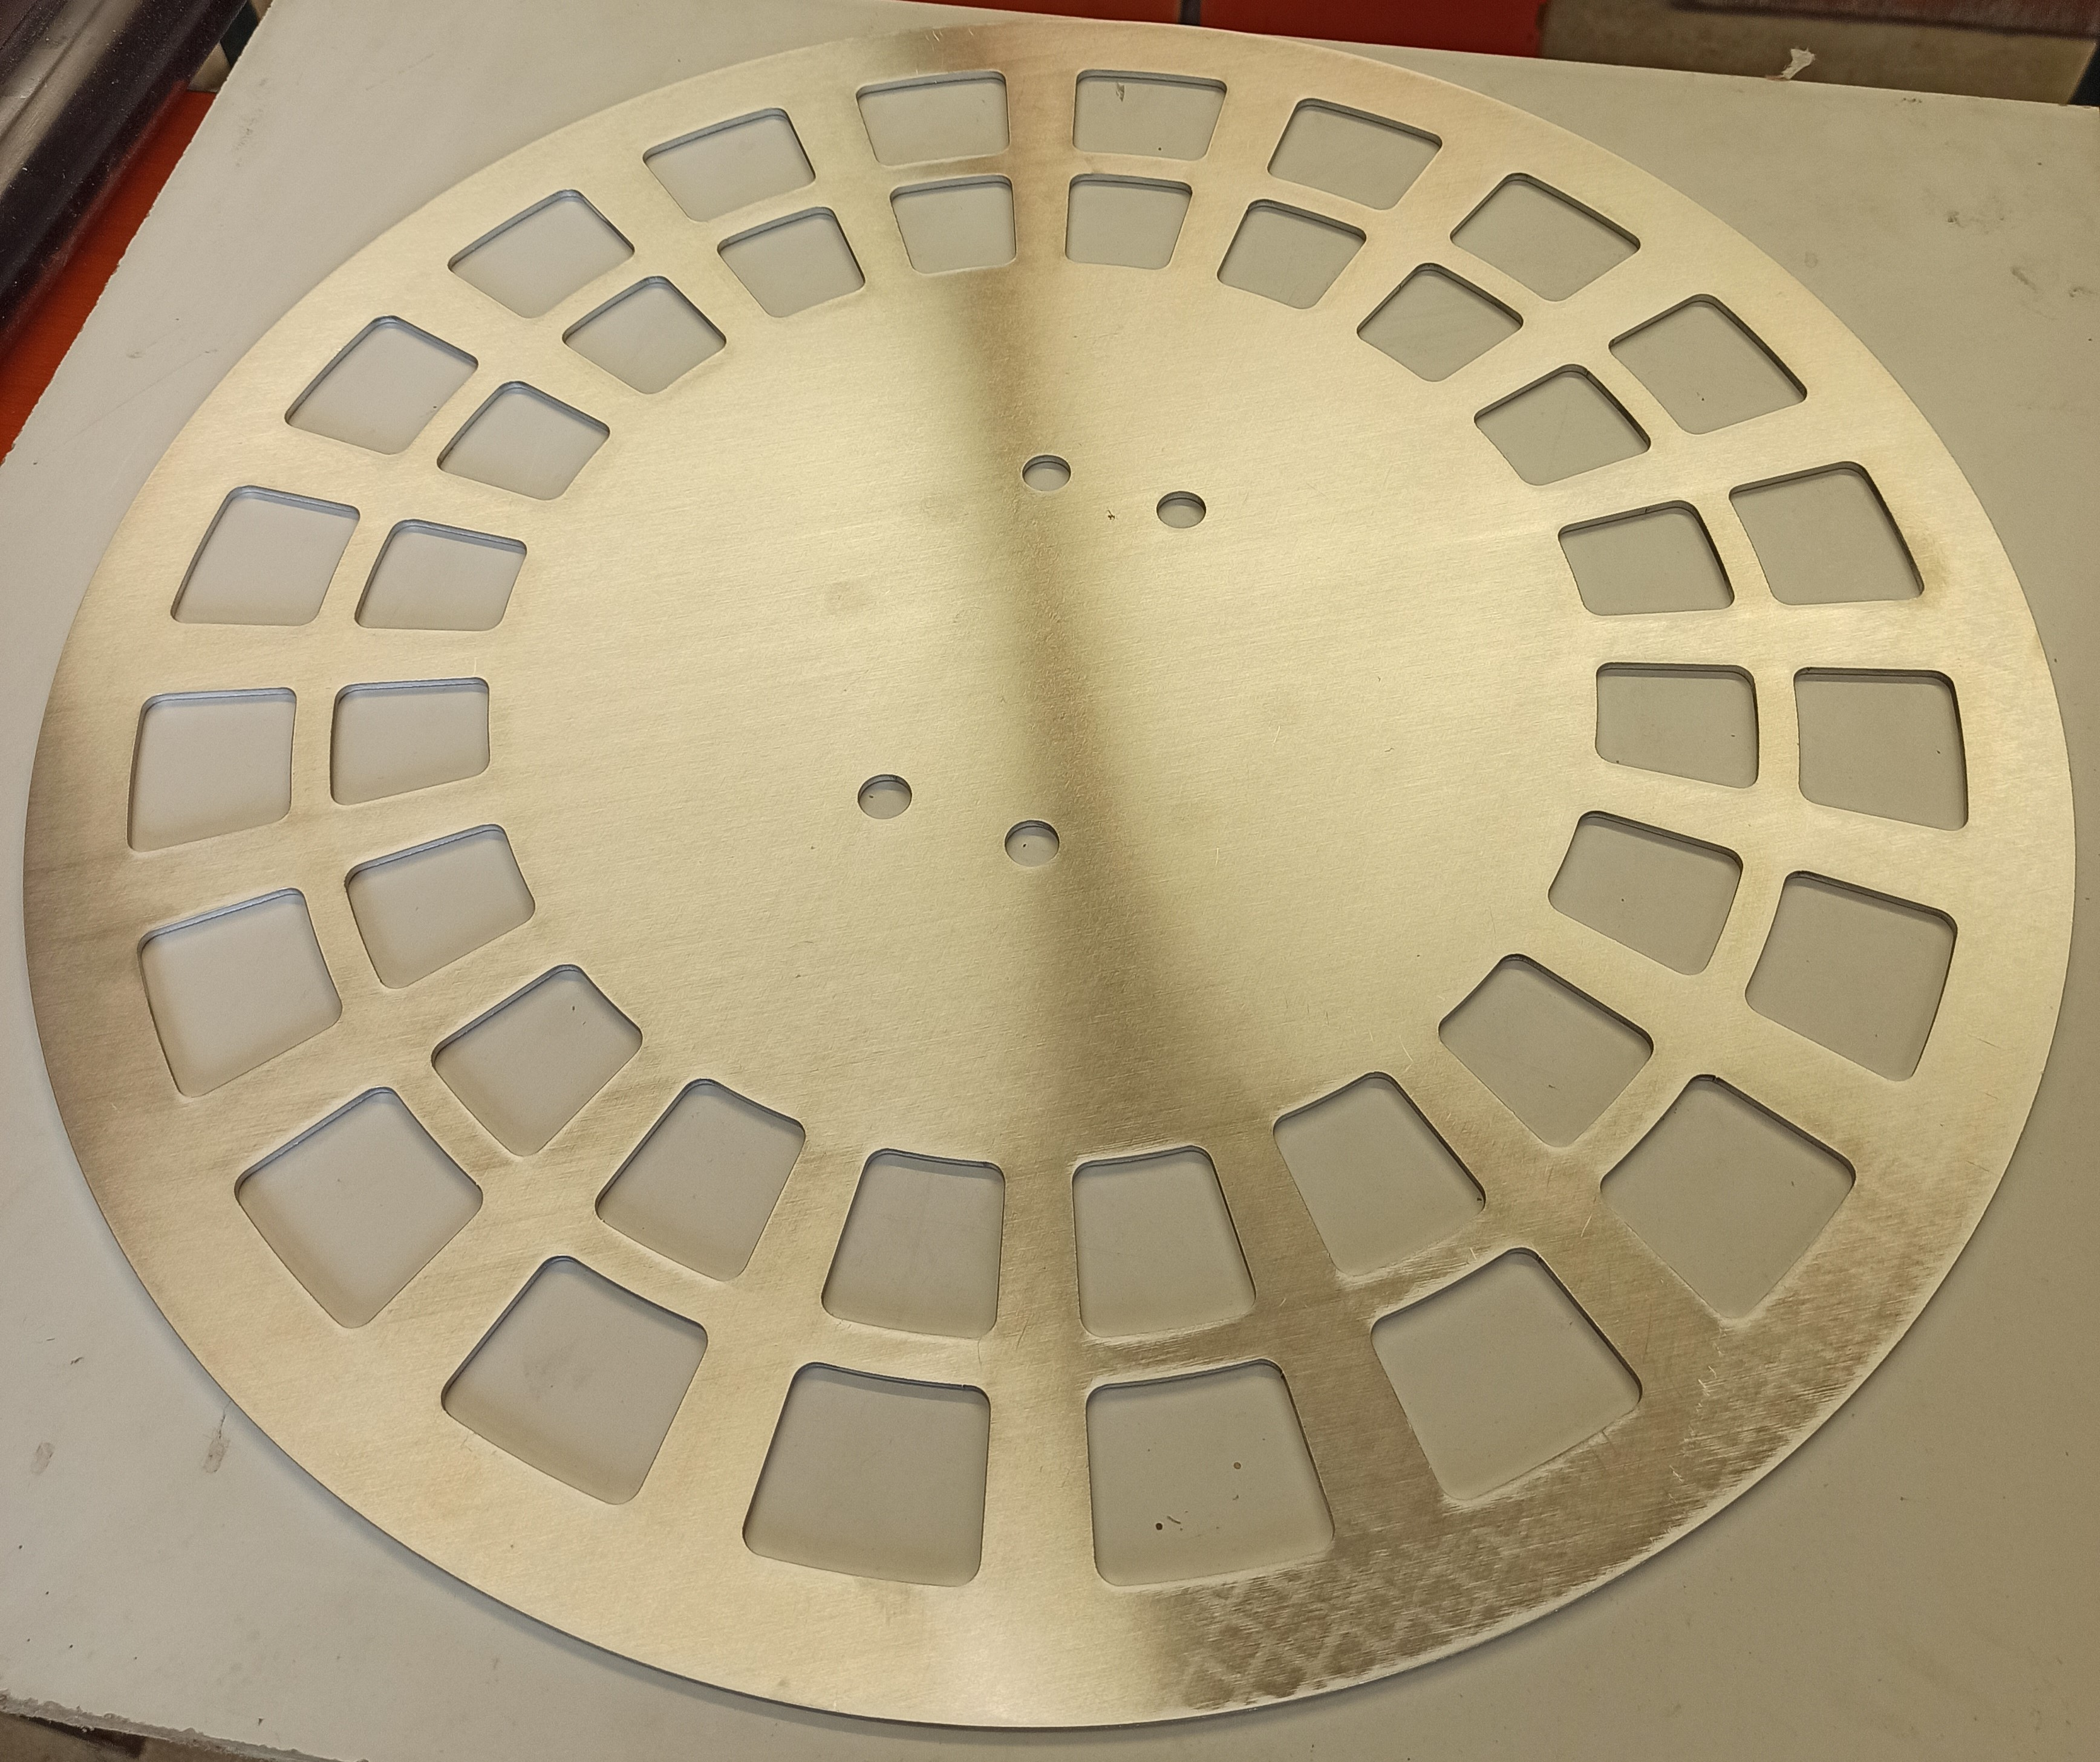
\includegraphics[width=\textwidth]{../ref/Reflektor.jpg}
	\caption{Reflektor der Wendelantenne}
	\label{fig:Reflektor}
\end{figure}

In der Mitte des Reflektors werden zwei Löcher mit einem Durchmesser von 13,5mm gebohrt an denen der Rohrflansch befestigt wird. 

Die Helix wurde real ebenso gebogen wie in der Simulation. Es wurde ein Aluminiumrohr mit einem Außendurchmesser von 18mm und einer Wandstärke von 2mm verwendet. Das Rohr hat eine Länge von ca. 5,2m und wurde zu einer Spirale gebogen, welche einen Durchmesser von 270mm, eine Höhe von ca. 1039,2mm und konsequent eine Steigung von 11,5° beziehungsweise einen Abstand zwischen den Windungen von 172,5mm hat.

\begin{figure}[h!]
	\centering
	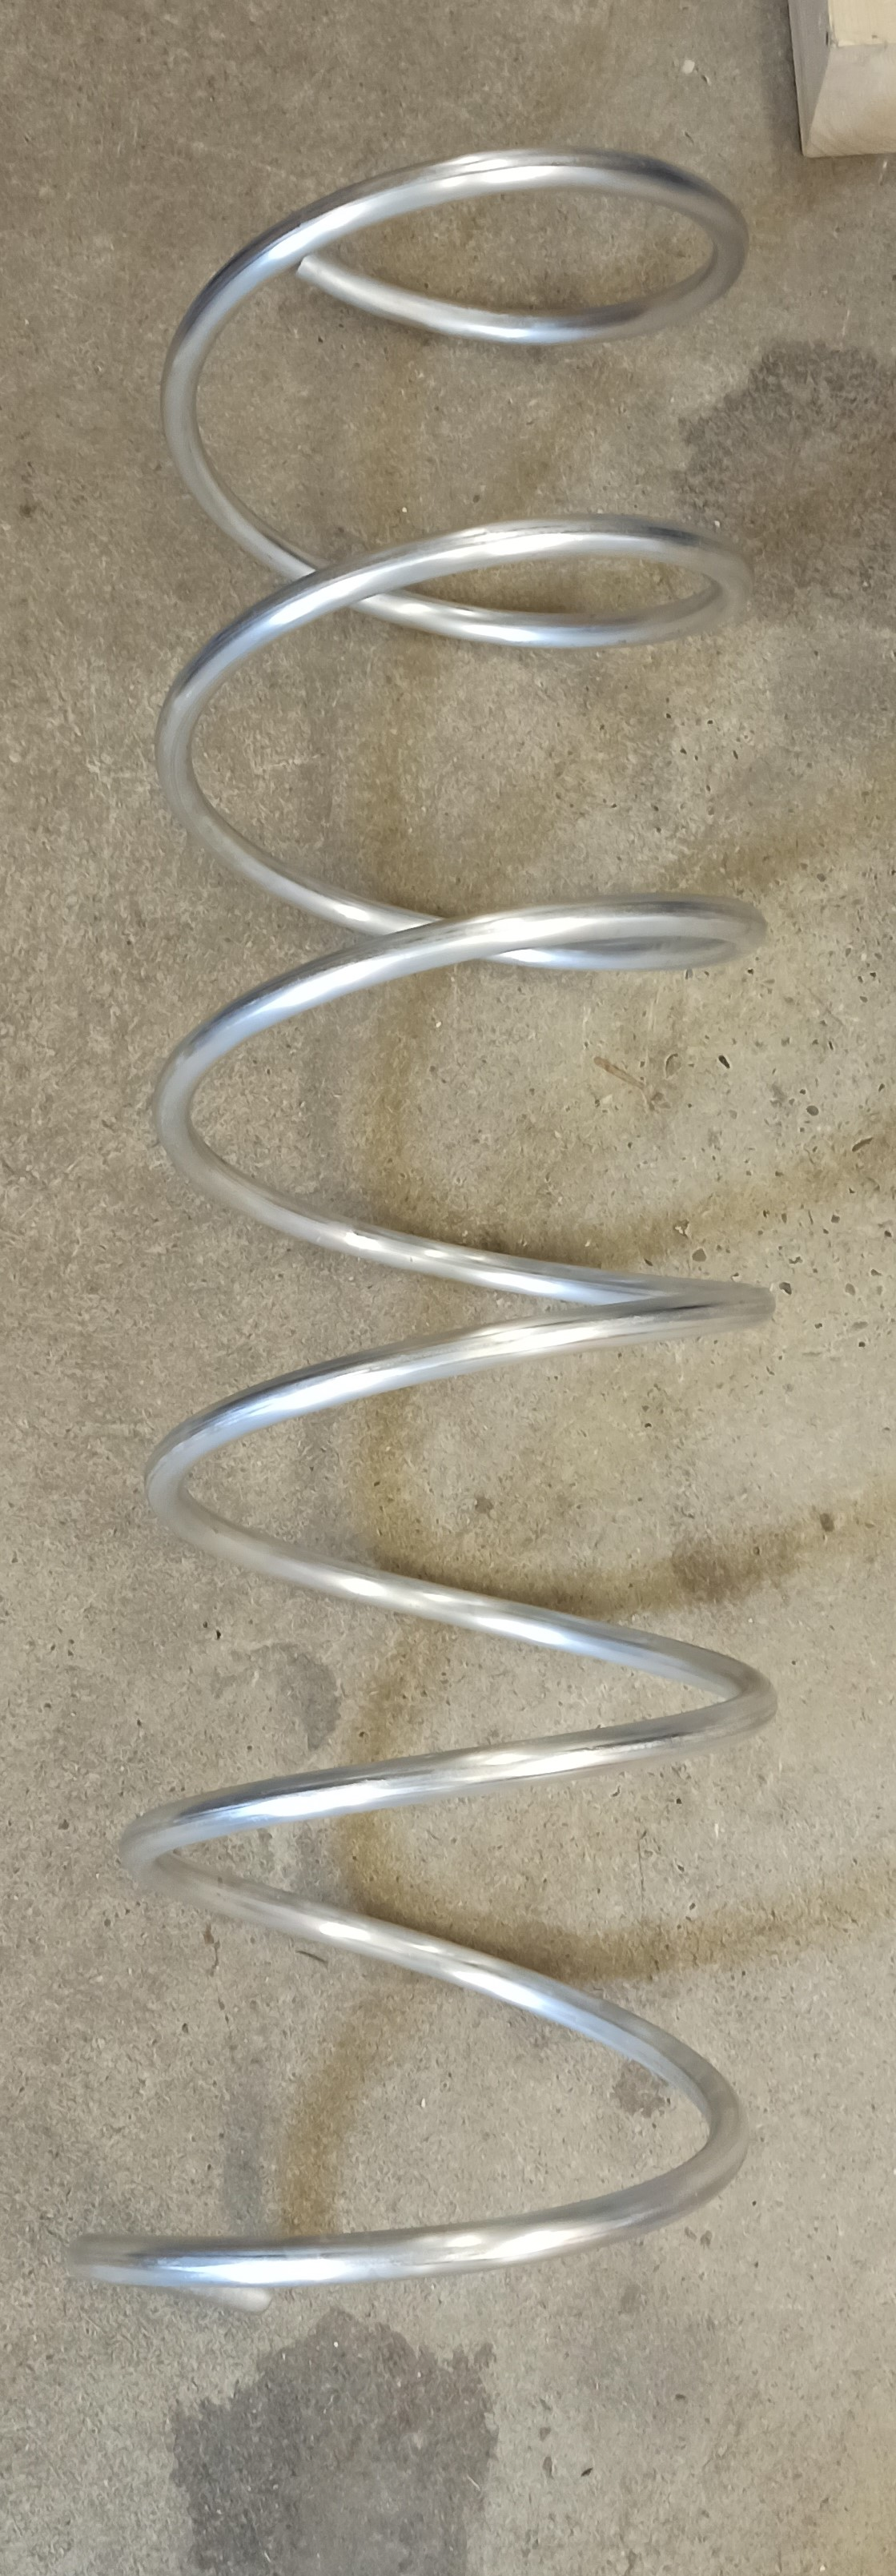
\includegraphics[width=5cm,angle=90]{../ref/Spirale.jpg}
	\caption{Das Herzstück der Wendelantenne: Die Helix}
	\label{fig:Spirale}
\end{figure}

Um die Helixantenne wasserdicht zu machen wurden kurz abgeschnittene Aluminiumrundlinge auf die Öffnungen des Helixrohres geschweißt. Am unteren Ende der Helix, an der der Innenleiter des Koaxialkabels befestigt wird, ist ein Gewinde in die Metallplatte geschnitten.

\begin{figure}[h!]
	\centering
	\includegraphics[width=\textwidth]{../ref/Deckel-oben.jpg}
	\caption{Aufgeschweißter Aluminiumrundling oben}
	\label{fig:Deckel-Helix-Oben}
\end{figure}

\begin{figure}[h!]
	\centering
	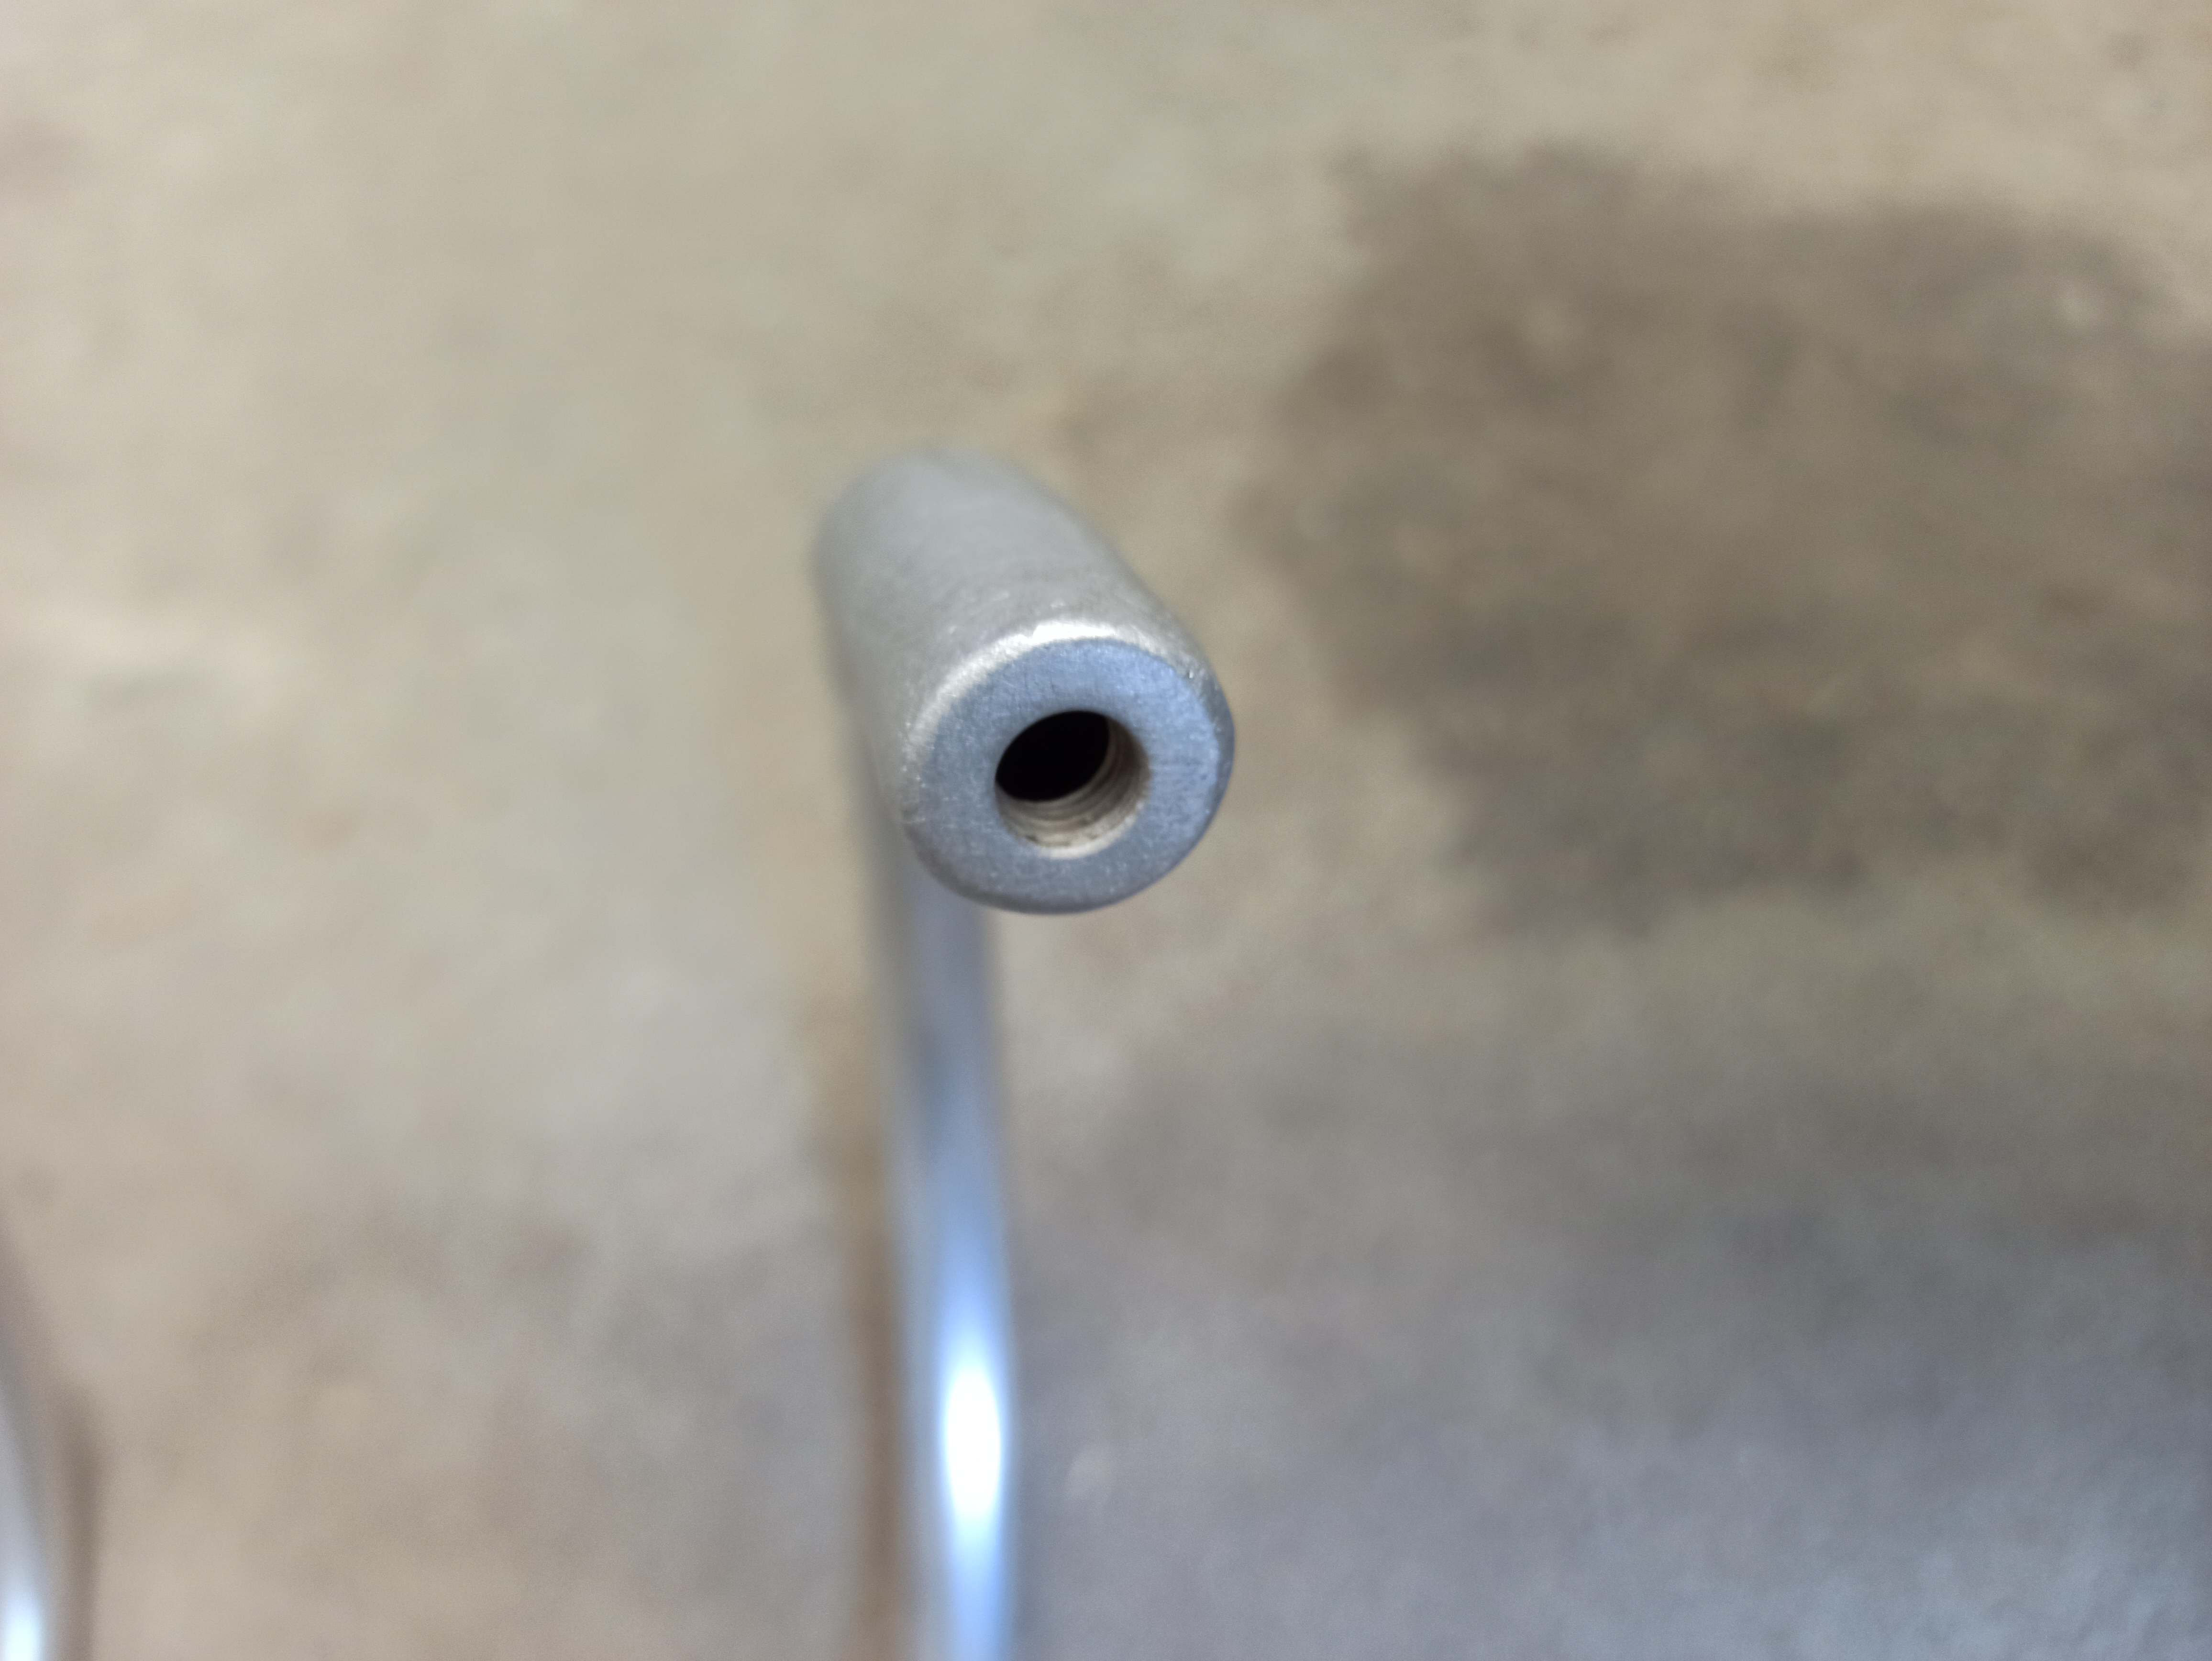
\includegraphics[width=\textwidth]{../ref/Anschluss-unten.jpg}
	\caption{Aufgeschweißter Aluminiumrundling unten (Befestigung des Innenleiters)}
	\label{fig:Deckel-Helix-Unten}
\end{figure}

Mithilfe dieses Gewindes kann ein Kabel durch einen Ringkabelschuh und eine Schraube montiert, und am Innenleiter der BNC-Buchse angelötet werden.

Um die PVC-Rohre vor Wasser zu schützen wurden Abdeckungen 3D-gedruckt. Durch die Verwendung eines speziellen Filaments vom Typ DuraPro ASA, ist das Resultat eine UV-resistente Rohrabdeckung. Durch diese Eigenschaft eignet sich dieses Filament exzellent für den Einsatz im Freien.

%Abdeckung fehlt

Die BNC-Buchse befindet sich direkt unter dem Ende der Spirale. Der Innenleiter wird, wie bereits erwähnt, an der Helix befestigt. Der Außenleiter wird mit dem Reflektor verschraubt.

%FEHLT: Bild der Buchse

\section{Anpassung}
Um eine einzelne Helixantenne anzupassen gibt es verschiedene Möglichkeiten. Eine weit verbreitete Option ist es, einen entsprechend dimensionierten Blechstreifen mit einer Länge von $\frac{\lambda}{4}$ entlang des unteren Endes der Helix zu montieren. Dieser agiert als Resonanztransformator und soll die Impedanz der Antenne auf einen Wert von 50$\Omega$ senken. Die Bandbreite der Wendelantenne bleibt bei dieser Anpassungsmethode erhalten.

Eine andere Möglichkeit, die Antenne anzupassen ist ein sogenannter $"$Power-Combiner$"$. Dieses Bauteil erlaubt es, Antennen mit einem Eingangswiderstand von 50 $\Omega$ zusammen zu schalten. Der springende Punkt bei dieser Art ist es, dass die Anpassung über rein reele Bauteile geschieht. Dies ermöglicht es, die Bandbreite der Antenne beizubehalten.



\section{Tests}
Tests im Freien, Messungen an Satelliten

\section{Erweiterung der Helixantenne als Array}
Nun wird die Helixantenne durch drei weitere identische Helixantennen erweitert, welche zusammen ein Array bilden. Hierbei ist der Abstand zwischen den einzelnen Antennen von Relevanz um den Gesamtgewinn zu maximieren.
Der Antennengewinn eines Antennenarrays bestehend aus vier identischen Helixantennen liegt in der Theorie bei dem vierfachen Antennengewinn einer einzelnen Wendelantenne, bzw. einer Helixantenne mit der vierfachen Windungszahl, also $4*6=24$.

Hierfür muss ein Gerüst designt und aufgebaut werden, welches vier solcher Antennen halten kann, sowie die neu entstehende Impedanz der Zusammenschaltung dieser Antenne angepasst werden. Anschließend müssen Tests durchgeführt werden, die den verbesserten Antennengewinn der Antenne belegen.

\subsection{Gerüst}

MATERIALLISTE

Als Gerüst wurde die Form eines $"$H$"$ gewählt. Da der Schwerpunkt des Gerüsts im Mittelpunkt liegt, wird das vom Rotor benötigte Moment minimiert. 

%Gegenüberstellung zu realem Gerüst
\begin{figure}[h!]
	\centering
	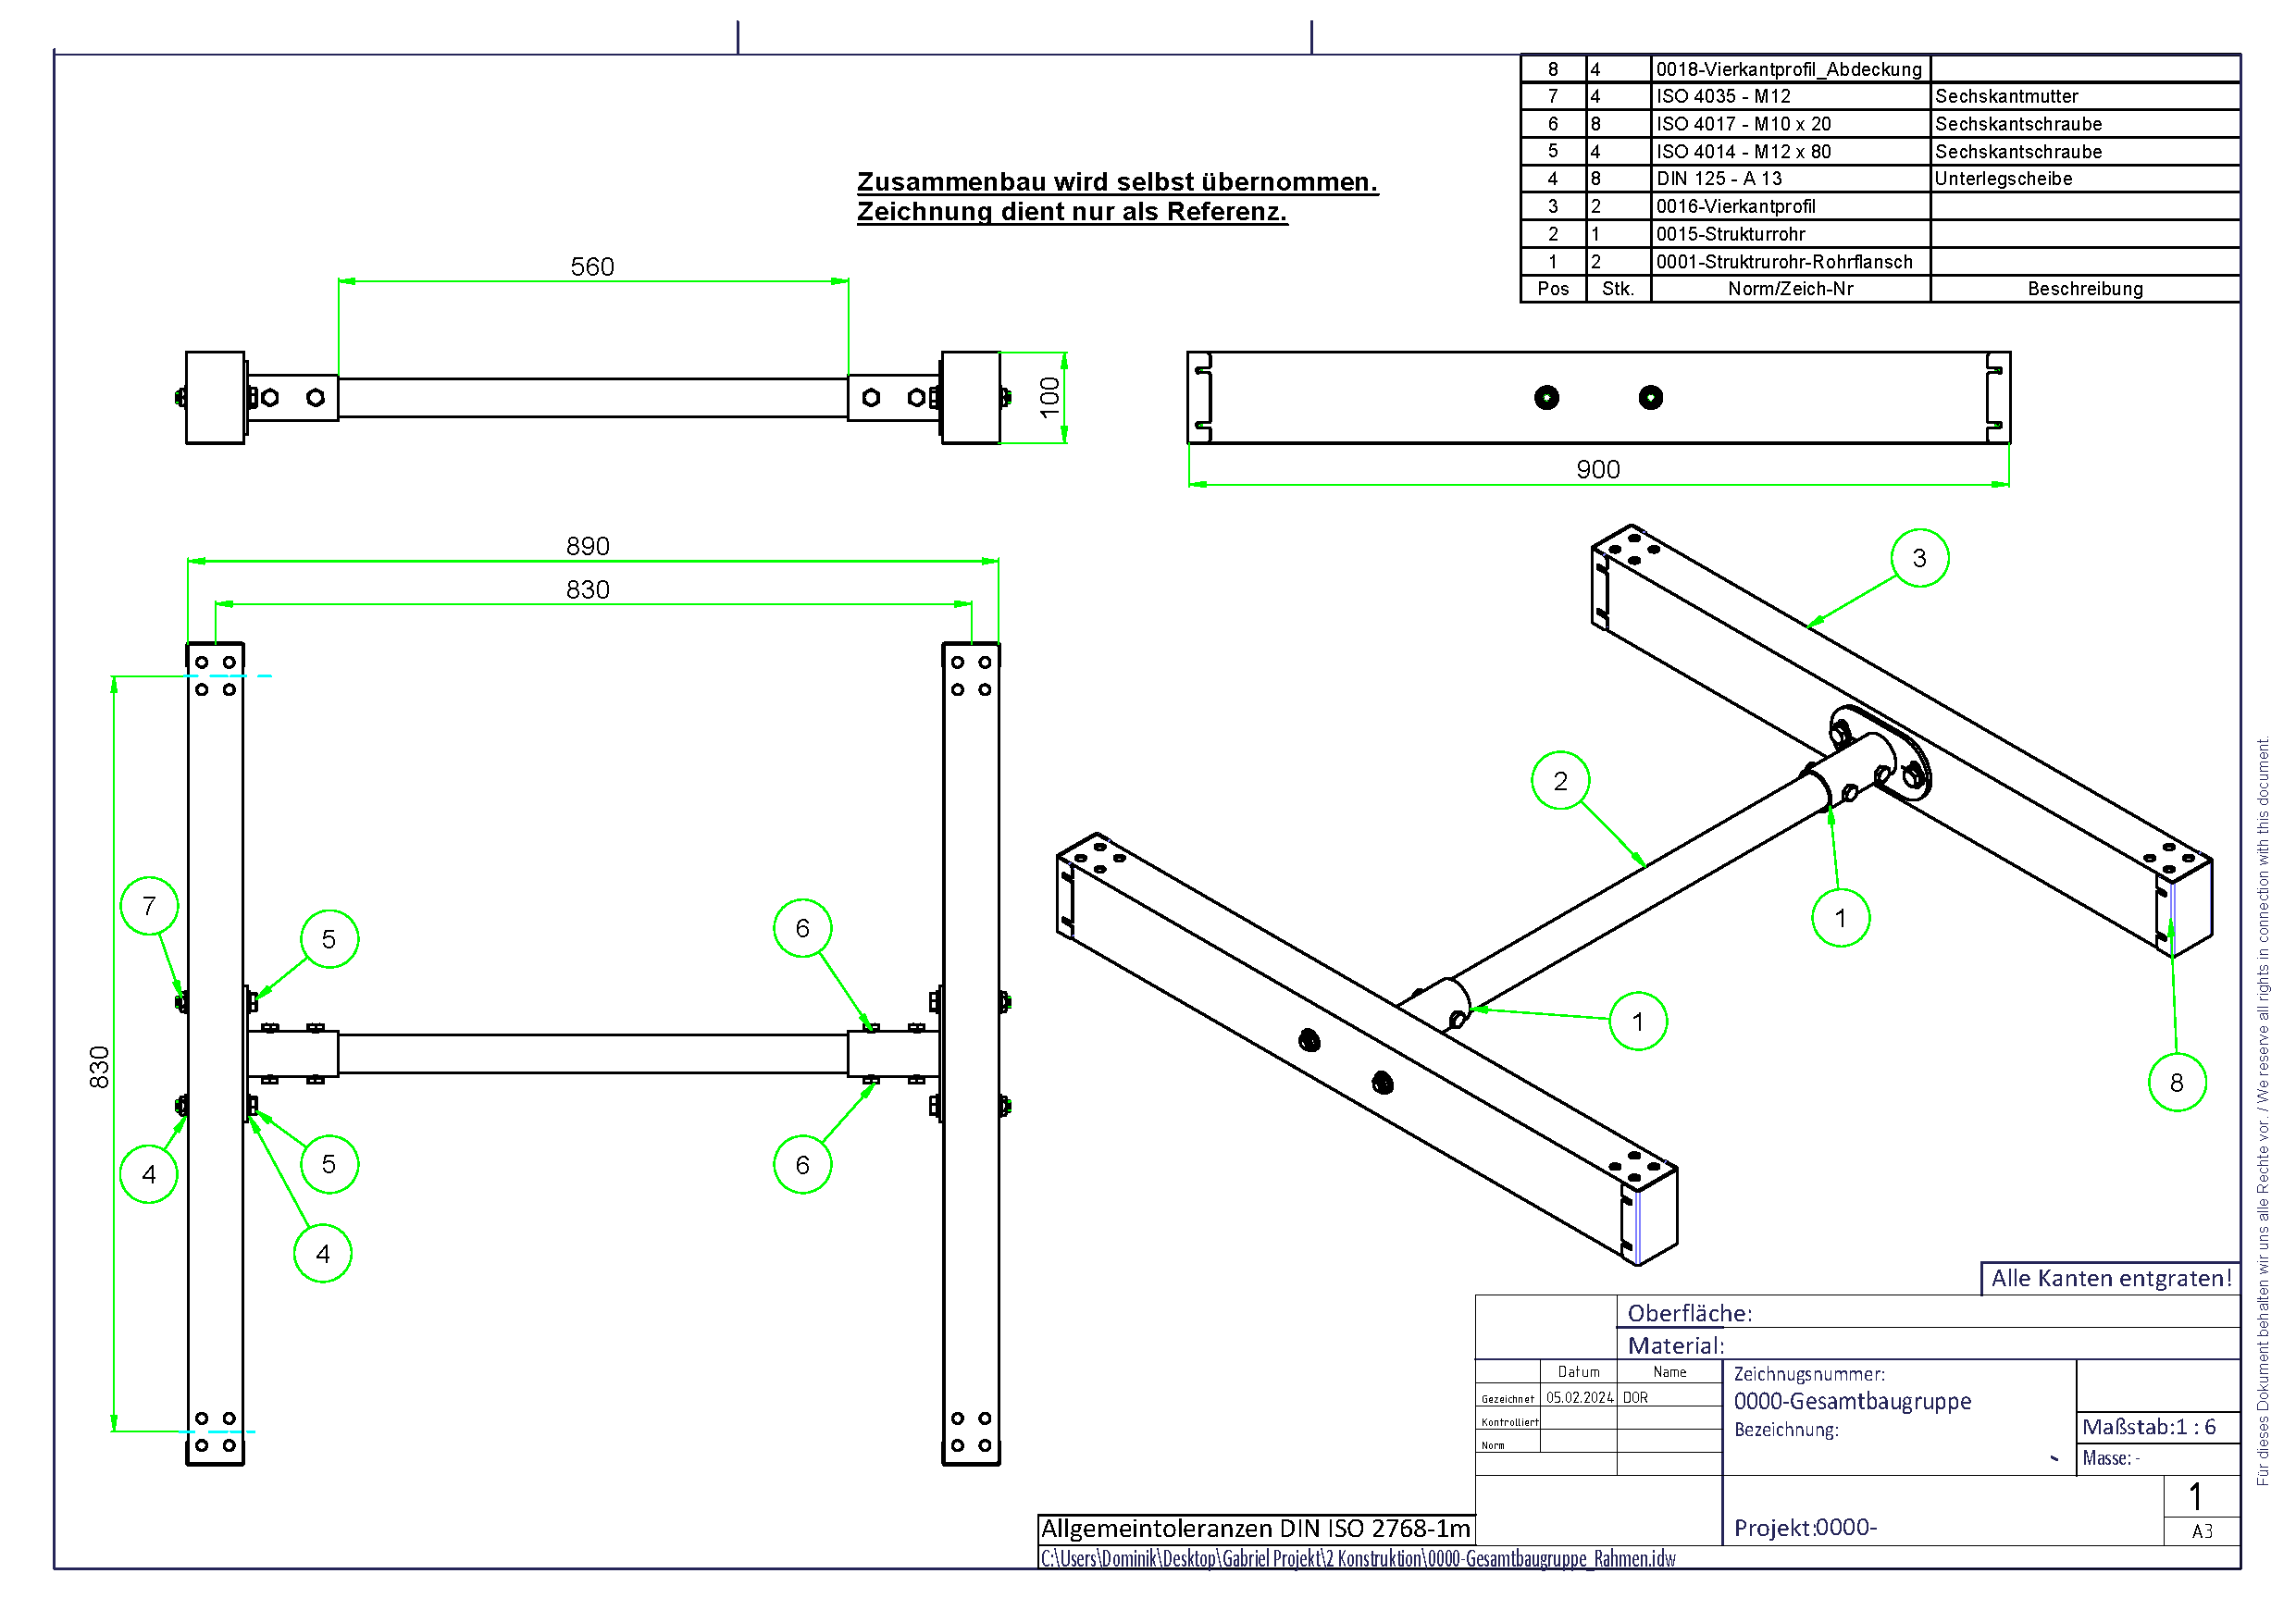
\includegraphics[keepaspectratio=true,scale=0.5]{../ref/0000-Gesamtbaugruppe_Rahmen.pdf}
	\caption{Bauplan des Gerüsts}
	\label{fig:Gerüst}
\end{figure}

Um eine komplette elektrische Isolierung der Antennen vom Gerüst zu ermöglichen, kommen Teflonplatten zum Einsatz. Diese verbinden die Antennen mit dem Aluminium-Vierkantprofil.

\begin{figure}[H]
	\begin{minipage}[b]{.4\linewidth} % [b] => Ausrichtung an \caption
		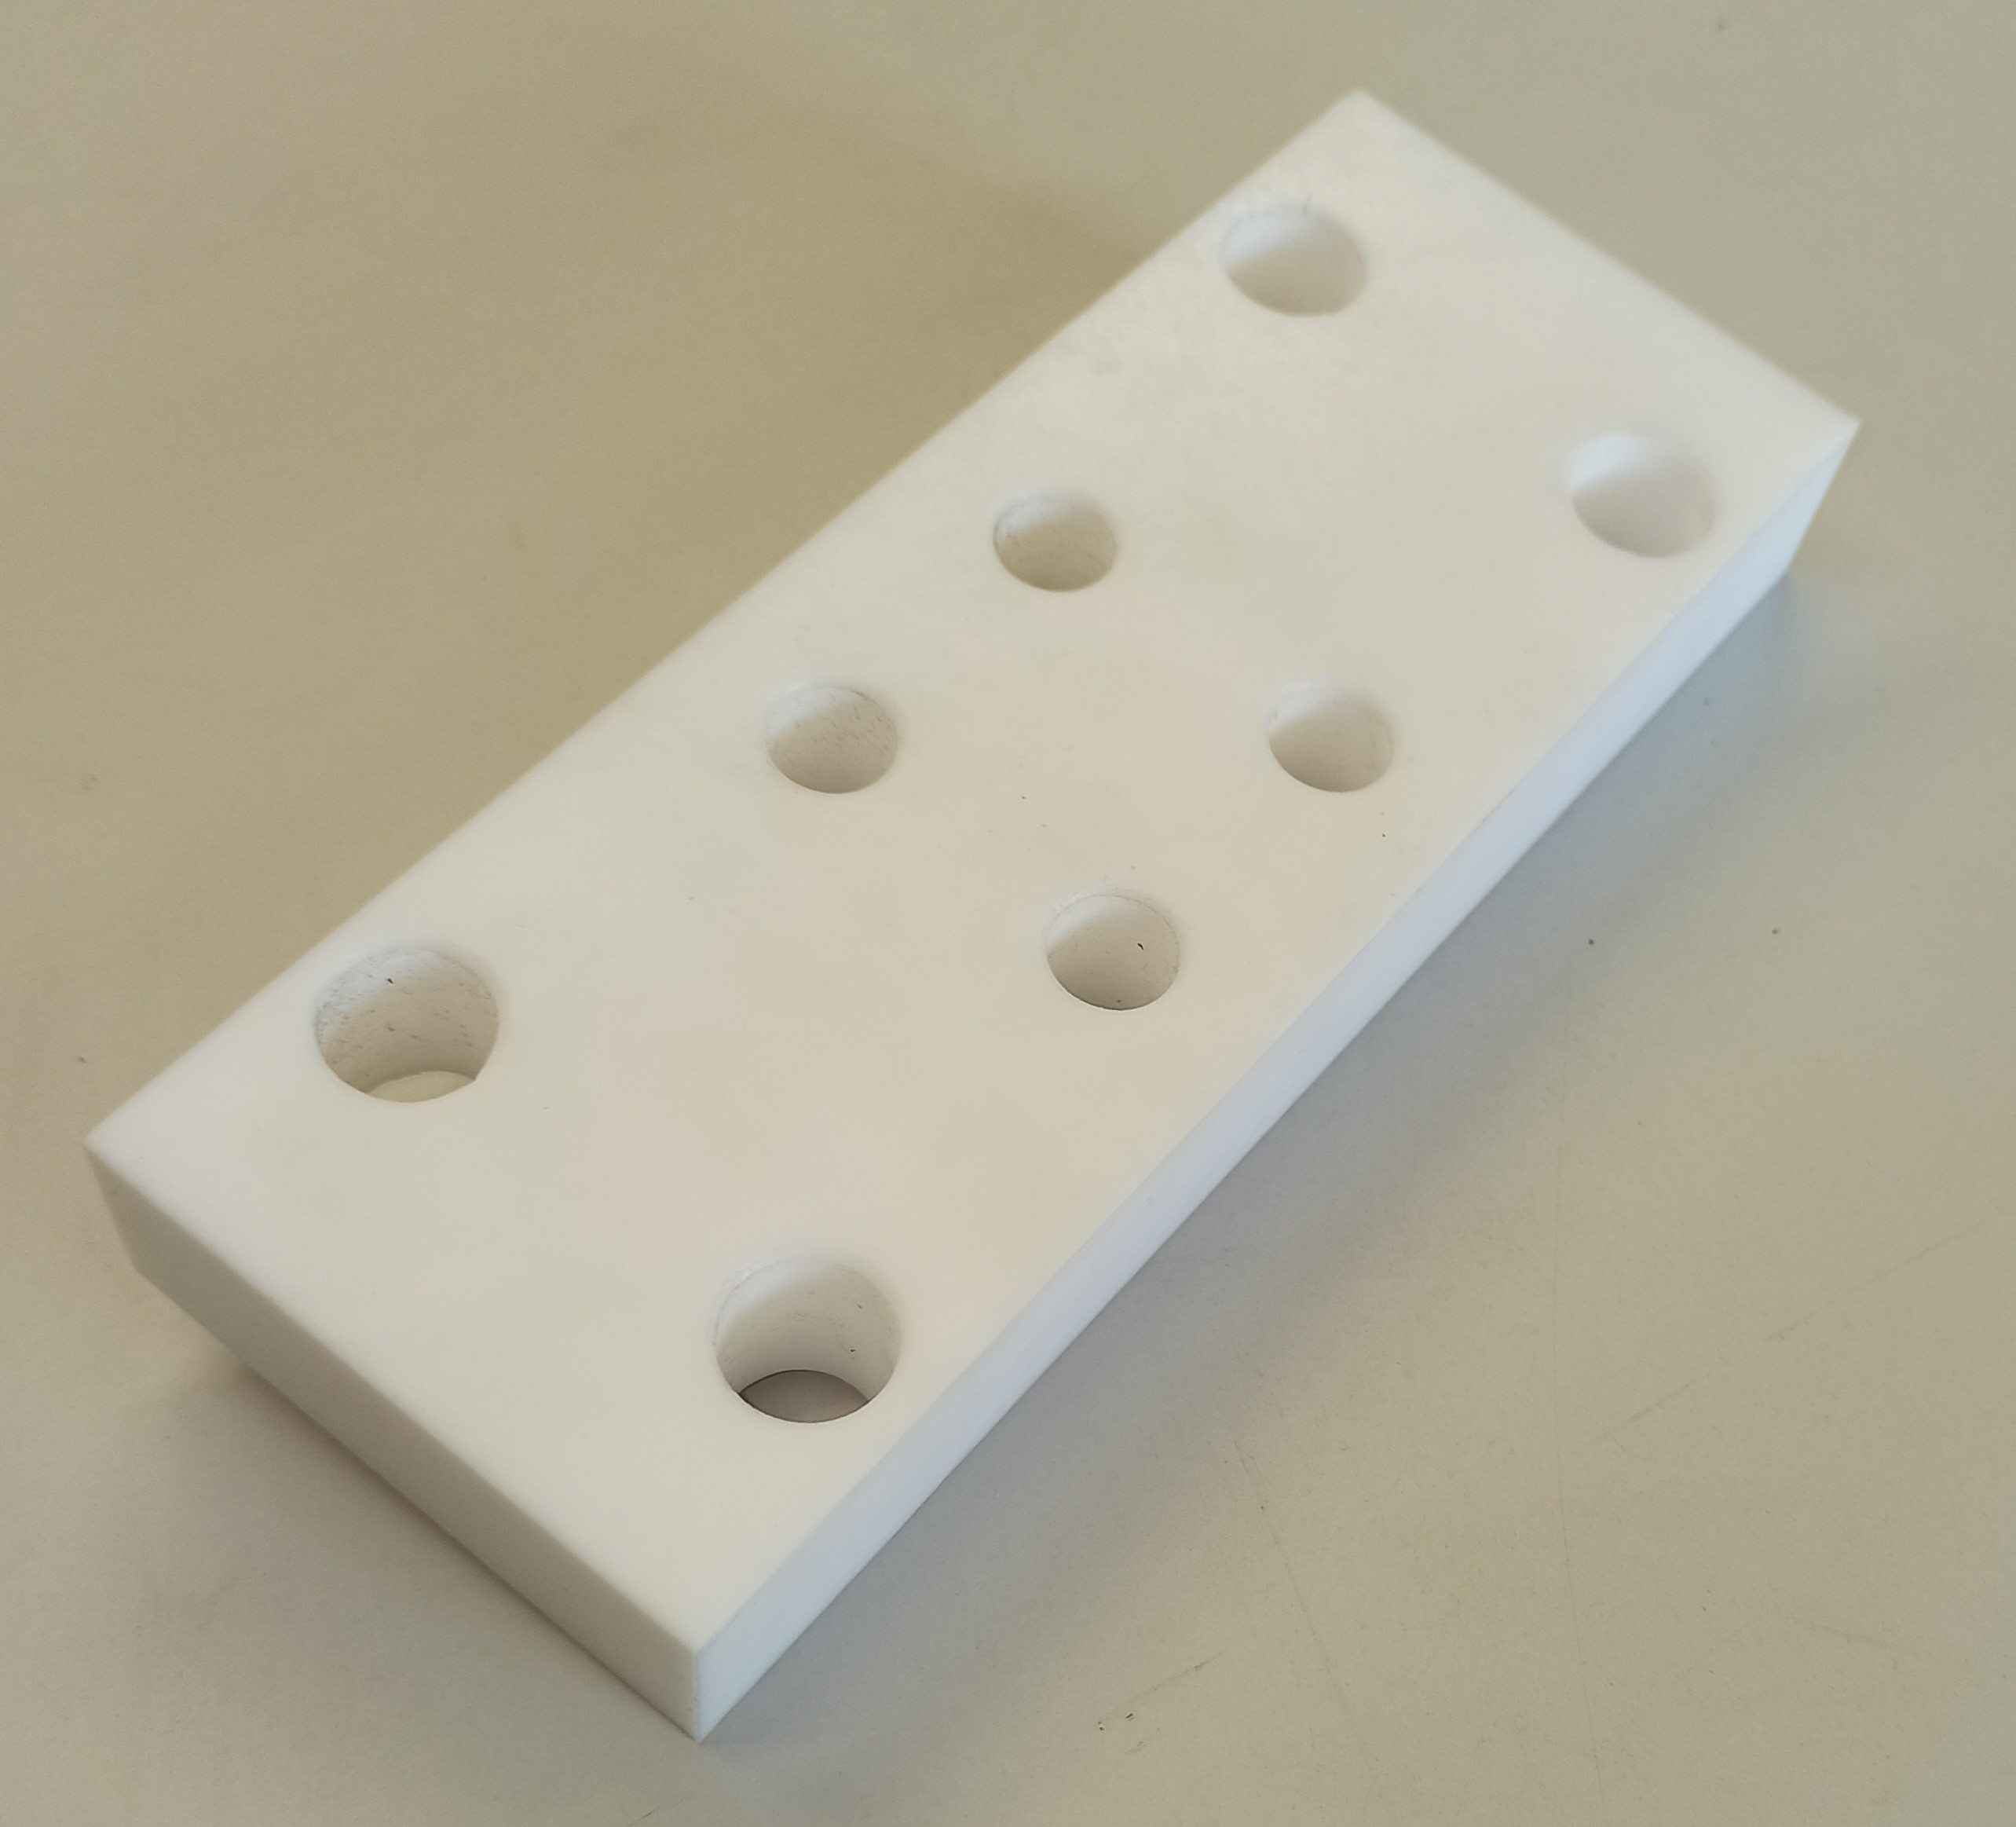
\includegraphics[width=\linewidth]{../ref/Teflon-Platte.jpg}
		\caption{Verbindende Teflonplatte}
		\label{fig:Teflonplatte}
	\end{minipage}
	\hspace{.1\linewidth}% Abstand zwischen Bilder
	\begin{minipage}[b]{.4\linewidth} % [b] => Ausrichtung an \caption
		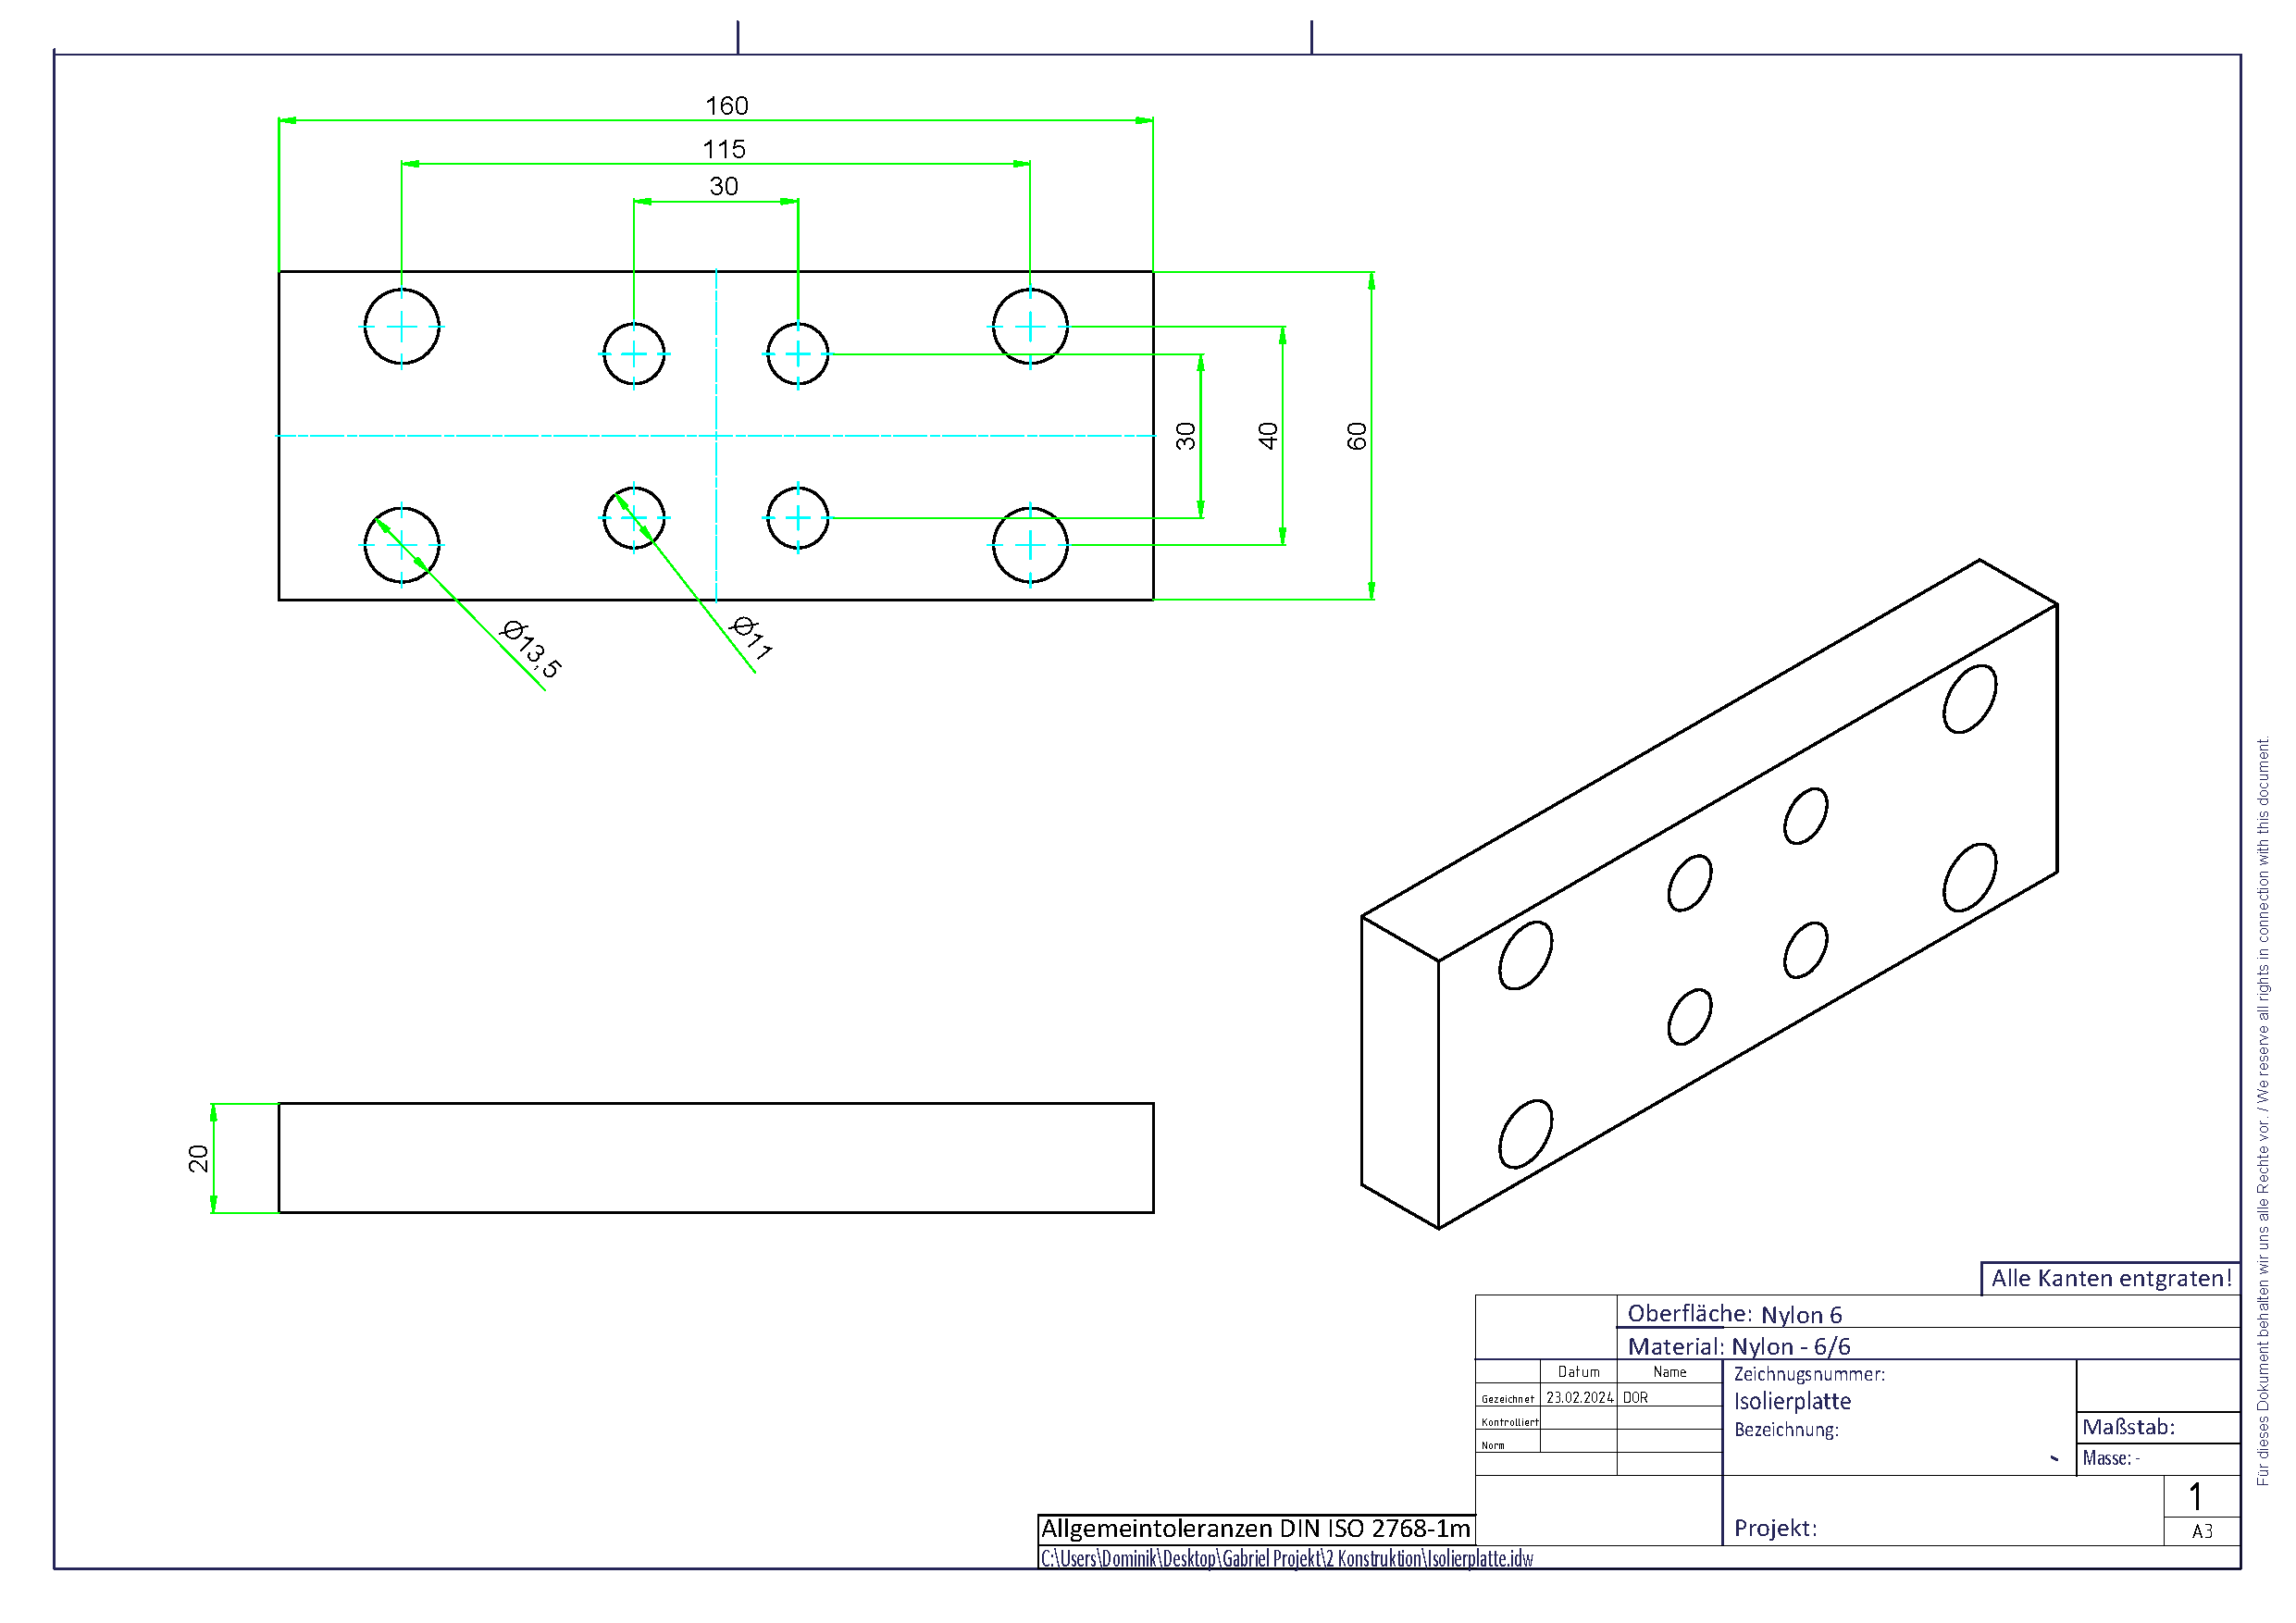
\includegraphics[width=\linewidth]{../ref/Isolierplatte.pdf}
		\caption{Zeichnung der Teflonplatte}
	\end{minipage}
\end{figure}

BILD DER VERBINDUNG

\subsection{Anpassung}
Da sich der Eingangswiderstand ändert, wenn vier solcher Antennen zusammen geschaltet werden, muss ein Anpassungsglied zwischen Koaxialkabel und Antennen eingesetzt werden. Hierbei wird eine Impedanz-Anpassungstechnik welche einfach zu implementieren ist. Diese besteht darin, einen Blechstreifen mit einer Länge von $\lambda/4$ an die erste Windung zu montieren. Dadurch wird die Impedanz auf 50$\Omega$ transformiert.

Der Anpassstreifen wurde mit zwei einzelnen Blechstreifen an dem unteren Ende der Helix angeschraubt.

BILD DER MONTAGE

Um nun vier Helixantennen zusammenzuschalten wird ein $\lambda/4$-Anpasstopf benötigt. Dieser verhält sich ähnlich wie ein Koaxialkabel, wobei das Verhältnis der Durchmesser zwischen Innenleiter und Außenleiter die Kapazität festlegt. Hierdurch kann der Wellenwiderstand angepasst werden.

BERECHNUNG

\cite{admin_lambda4_2016}

Es wurde hierbei die Variante mit einem viereckigen Außenleiter und einem runden Innenleiter angewendet, da sich die BNC-Buchsen an dem Vierkantrohr besser befestigen lassen.\\
Wird in die zuvor genannten Formeln eingesetzt, so erhält man die folgenden Ergebnisse.

BERECHNUNG



\subsection{Test}

Tests mit anderer Antenne im freien Feld